%%%%%%%%%%%%%%%%%%%%%%%%%%%%%%%%%%%%%%%%%%%%%%%%%%%%%%%%%%%%%%%%%%%%%%%%%%
%%%%%%%%%%%%%%%%%%%%%%%%%%%%%%%%%%%%%%%%%%%%%%%%%%%%%%%%%%%%%%%%%%%%%%%%%%
\clearpage{}
\section{Determination of signal yield from a fit to the \texorpdfstring{$m_{jj}/m_J$}{dijet/merged jet invariant mass} distribution}
\label{sec:mjj_fit}
We extract the diboson signal yield from an unbinned maximum
likelihood fit to the dijet invariant mass distribution in the data.
Tables~\ref{tab:mjj_shapes_and_normalization},~\ref{tab:mJ_shapes_and_normalization} show how the shape of
each component is determined, and what constraints are applied to fit
for the normalization (while a more involved discussion of how each PDF parameter is treated is given in Section~\ref{sec:individualProcesses}).
The fit output is summarized in
Table~\ref{table:FitTotalsAndComparisons}. The main sources of
systematics error are the uncertainties in the modeling/determining parameters of individual Pdf as well as
the jet energy scale (JES) uncertainty.
%%%%%%%%%%%%%%%%%%%%%%%%%%%%%%%%%%%%%%%%%%%%%%%%%%%%%%%%%%%%
\begin{table}[!htbp]
  \begin{center}
 \caption{Determination of the $m_{jj}$ shape and normalization. External constraints are assumed Gaussian.}  
 \label{tab:mjj_shapes_and_normalization} 
 \begin{tabular} {l  c  l}
   \hline \hline
   Process                &    Shape     & External constraint on normalization\\ \hline
   V plus jets            &    PDF/data   & Constrained: $\pm$ 5\%~\cite{MCFM} \\
   Diboson                &    PDF        & Unconstrained \\ 
   Top                    &    PDF/data        & Constrained: $\pm$ 7\% ~\cite{Kidonakis:2010dk,Kidonakis:2010tc,Kidonakis:2011wy,Kidonakis:2010ux}\\ 
   $WH(150)\to bb$        &    PDF        & Fixed to expectation or neglected \\ 
   Multijet               &    data      & Constrained: \MET fit in data $\pm$  50\%  \\\hline \hline
 \end{tabular}
\end{center}
\end{table}
%%%%%%%%%%%%%%%%%%%%%%%%%%%%%%%%%%%%%%%%%%%%%%%%%%%%%%%%%%%%
%%%%%%%%%%%%%%%%%%%%%%%%%%%%%%%%%%%%%%%%%%%%%%%%%%%%%%%%%%%%
\begin{table}[!htbp]
  \begin{center}
 \caption{Determination of the $m_J$ shape and normalization. External constraints are assumed Gaussian. The term sideband refers to diboson resonance corrections and expected yields expected based on the $t\bar{t}$ control region studies (Sec.~\ref{sec:ttbar_merged}).}  
 \label{tab:mJ_shapes_and_normalization} 
 \begin{tabular} {l  c  l}
   \hline \hline
   Process                &    Shape     & External constraint on normalization \\ \hline
   V plus jets            &    data      & Effectively Unonstrained: $\pm$ 50\% \\
   Diboson                &    PDF/sideband       & Unconstrained \\ 
   Top                    &    PDF/sideband       & Constrained: $\pm$ 8-10\% - sideband \\
 \hline \hline
 \end{tabular}
\end{center}
\end{table}
%%%%%%%%%%%%%%%%%%%%%%%%%%%%%%%%%%%%%%%%%%%%%%%%%%%%%%%%%%%%
%%%%%%%%%%%%%%%%%%%%%%%%%%%%%%%%%%%%%%%%%%%%%%%%%%%%%%%%%%%%%%%
%%%\begin{table}[!htbp]
%%%  \begin{center}
%%% \caption{Event yields determined from a likelihood fit
%%% to the data. The total uncertainty takes into
%%% account the correlations among individual components.}
%%% \label{tab:mjj_shapes_and_normalization}
%%% \begin{tabular} {l  c  c c c }
%%%   \hline \hline
%%%   Process             &    \multicolumn{2}{c}{Muon channel} & \multicolumn{2}{c}{Electron channel} \\  
%%%\hline
%%%                       &    2 jets              &  3 jets              & 2 jets             &  3 jets\\  
%%%\hline
%%%   W+jets              &    53231  $\pm$  466   &  12551 $\pm$  331    &  30075 $\pm$ 115   &  8725 $\pm$  273\\
%%%   Dibosons            &    1087 $\pm$  98      &  339 $\pm$  49       &  642 $\pm$  61     &  173 $\pm$  17\\
%%%   $t\bar{t}$          &    3973  $\pm$  238    &  7738 $\pm$  330     &  2313 $\pm$ 143    &  3939 $\pm$  216\\
%%%   Single top          &    1545  $\pm$  76     &  873 $\pm$  43       &  858 $\pm$  43     &  489 $\pm$  24\\
%%%   Drell-Yan+jets      &    1362 $\pm$  58      &  417 $\pm$  18       &  993 $\pm$  43     &  341 $\pm$  15\\
%%%   Multijet            &    84 $\pm$  256       &  0 $\pm$ 90          &  4040 $\pm$ 1170   &  334 $\pm$  160\\
%%%\hline
%%%   Total from fit      &    61281 $\pm$ 290     &  21918 $\pm$ 183     &  38923 $\pm$ 227   &  14000 $\pm$ 141\\
%%%   Data                &    61153               &  22030               &  38973             &  14145 \\
%%%\hline
%%%\multicolumn{5}{c}{in region $(123\,\text{GeV} < m_{jj} < 186\,\text{GeV})$} \\
%%%\hline
%%%  Total from fit & 12921 $\pm$ 118 & 7021 $\pm$ 91 & 7909 $\pm$ 92 & 4297 $\pm$ 70\\
%%%  Data & 12761 & 7111 & 8023 & 4438 \\
%%%\hline \hline
%%% \end{tabular}
%%%\end{center}
%%%\end{table}
%%%%%%%%%%%%%%%%%%%%%%%%%%%%%%%%%%%%%%%%%%%%%%%%%%%%%%%%%%%%%%%
\subsection{Fit results}
\label{sec:mjj_2jetfit}
The results of the fit are shown 
in Figs.~\ref{fig:mjj_2jet_mu},~\ref{fig:mjj_2jet_el} for the anti-btagged dijet (standard) selection,
Figs.~\ref{fig:mjj_2jet_mu_btag},~\ref{fig:mjj_2jet_el_btag} for the btagged dijet selection and Figs.~\ref{fig:mJ_mu_boosted},~\ref{fig:mJ_el_boosted} for the boosted events. 
A clear peak from the Standard Model electroweak diboson 
WW/WZ production can be seen. 
The mean mass, resolution and yield for the diboson events are 
consistent with the Standard Model predictions computed up to 
the next-to-leading order (NLO) in perturbation theory.
These consistency checks give us confidence in the analysis procedures.
The fit results are tabulated below.
%%%%%%%%%%%%%%%%%%%%

\underline{Muons, Anti-Btagged, Dijet Regime:}
{\tiny
\input{log_Diboson_Muon.log}
}

\underline{Electrons, Anti-Btagged, Dijet Regime:}
{\tiny
\input{log_Diboson_Electron.log}
}

\underline{Muons, Btagged, Dijet Regime:}
{\tiny
\input{log_Diboson_Muon_Btag.log}
}

\underline{Electrons, Btagged, Dijet Regime:}
{\tiny
\input{log_Diboson_Electron_Btag.log}
}

\underline{Muons, Boosted Regime:}
{\tiny
\input{log_Diboson_Muon_boosted.log}
}

\underline{Electrons, Boosted Regime:}
{\tiny
\input{log_Diboson_Electron_boosted.log}
}

%%%%%%%%%%%%%%%%%%%%
%%%%%%%%%%%%%%%%%%%%
%%%%%%%%%%%%%%%%%%%%
%%%%%%%%%%%%%%%%%%%%
\begin{figure}[h!]
  {\centering
    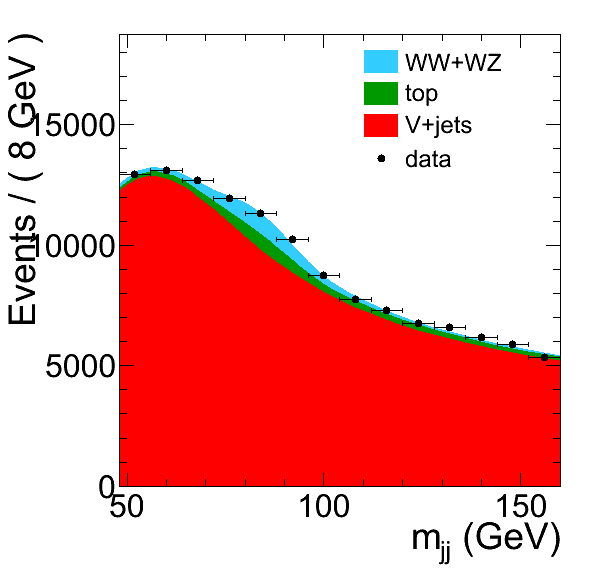
\includegraphics[width=0.49\textwidth]{figs/mjjfit/Dibosonlnujj_muon_Stacked.png}
    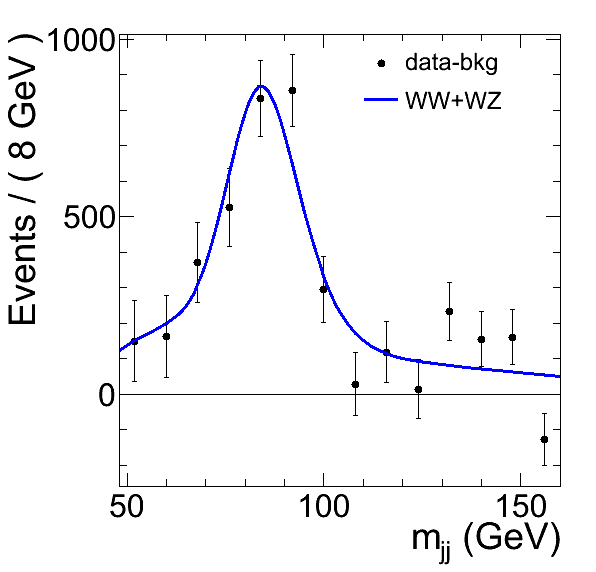
\includegraphics[width=0.49\textwidth]{figs/mjjfit/Dibosonlnujj_muon_Subtracted.png}
    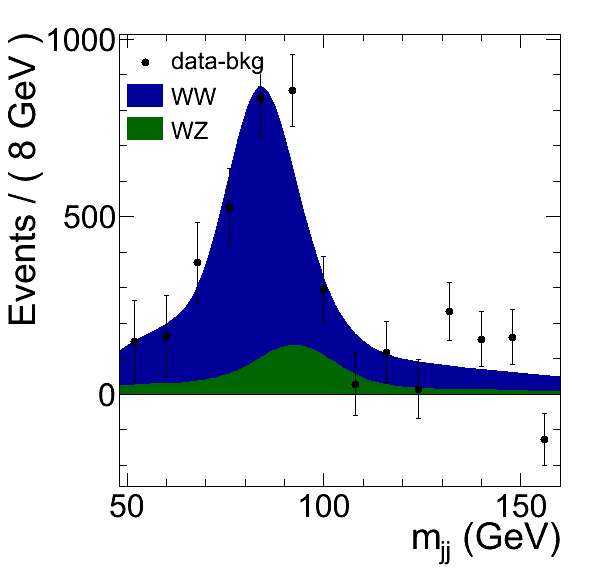
\includegraphics[width=0.49\textwidth]{figs/mjjfit/Dibosonlnujj_muon_Split.png}
    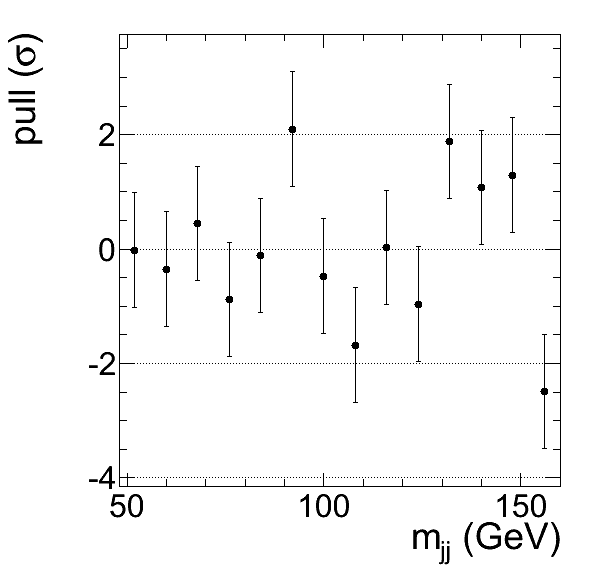
\includegraphics[width=0.49\textwidth]{figs/mjjfit/Dibosonlnujj_muon_Pull.png}
    \caption{Distribution of the dijet invariant mass for the (non-boosted, anti-btagged) 2-jet events in muon data and fit shapes: 
      (upper left) All background components stacked together, 
      (upper right) Data minus all backgrounds except diboson,
      (lower left) Data minus all backgrounds except diboson with $WW$ and $WZ$ contributions shown separately,
      (lower right) normalized residual between data and MC. The vertical dotted lines
      indicate the mass interval excluded from the fit.}
    \label{fig:mjj_2jet_mu}}
\end{figure}
%%%%%%%%%%%%%%%%%%%%
%%%%%%%%%%%%%%%%%%%%
\begin{figure}[h!]
  {\centering
    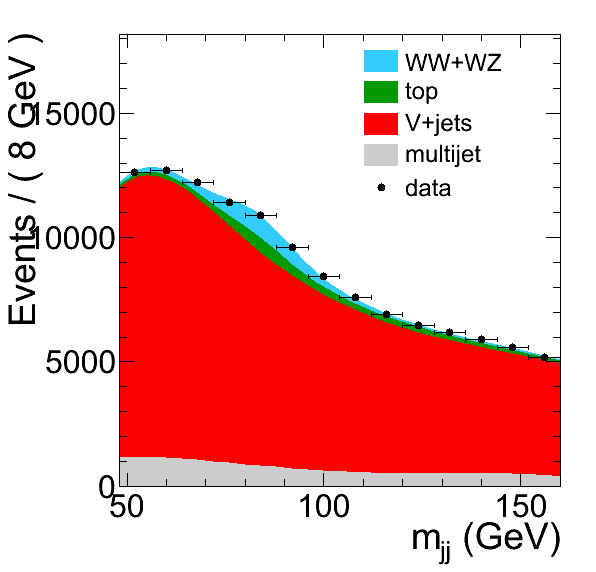
\includegraphics[width=0.49\textwidth]{figs/mjjfit/Dibosonlnujj_electron_Stacked.png}
    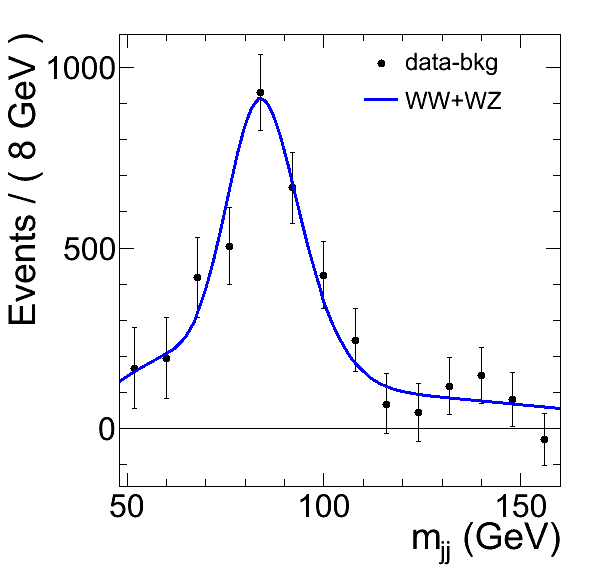
\includegraphics[width=0.49\textwidth]{figs/mjjfit/Dibosonlnujj_electron_Subtracted.png}
    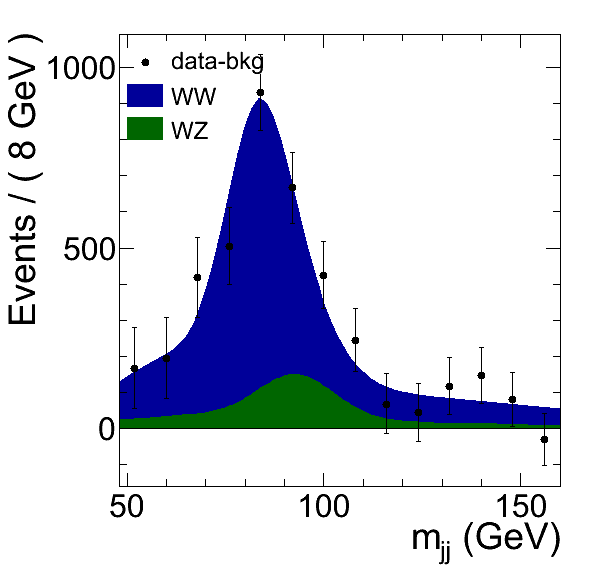
\includegraphics[width=0.49\textwidth]{figs/mjjfit/Dibosonlnujj_electron_Split.png}
    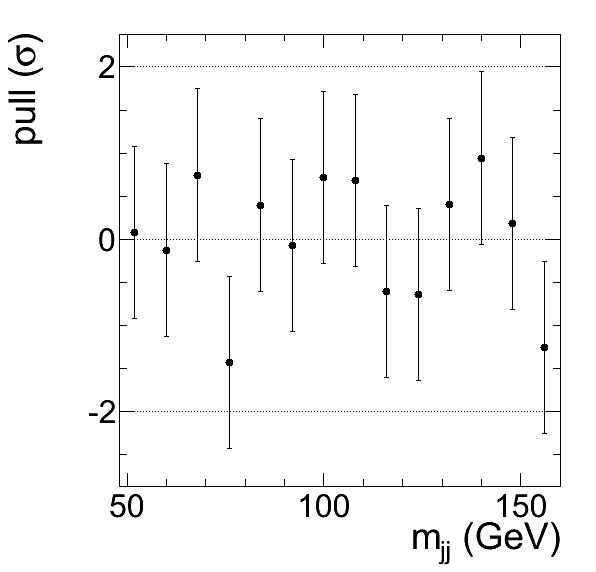
\includegraphics[width=0.49\textwidth]{figs/mjjfit/Dibosonlnujj_electron_Pull.png}
    \caption{Distribution of the dijet invariant mass for the (non-boosted, anti-btagged) 2-jet events in electron data and fit shapes: 
      (upper left) All background components stacked together, 
      (upper right) Data minus all backgrounds except diboson,
      (lower left) Data minus all backgrounds except diboson with $WW$ and $WZ$ contributions shown separately,
      (lower right) normalized residual between data and MC. The vertical dotted lines
      indicate the mass interval excluded from the fit.}
    \label{fig:mjj_2jet_el}}
\end{figure}
%%%%%%%%%%%%%%%%%%%%
%%%%%%%%%%%%%%%%%%%%%
\begin{figure}[h!]
  {\centering
    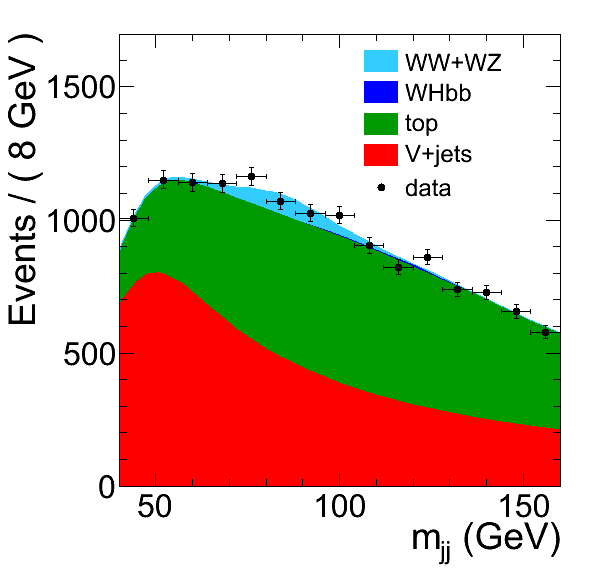
\includegraphics[width=0.49\textwidth]{figs/mjjfit/DibosonBtaglnujj_muon_Stacked.png}
    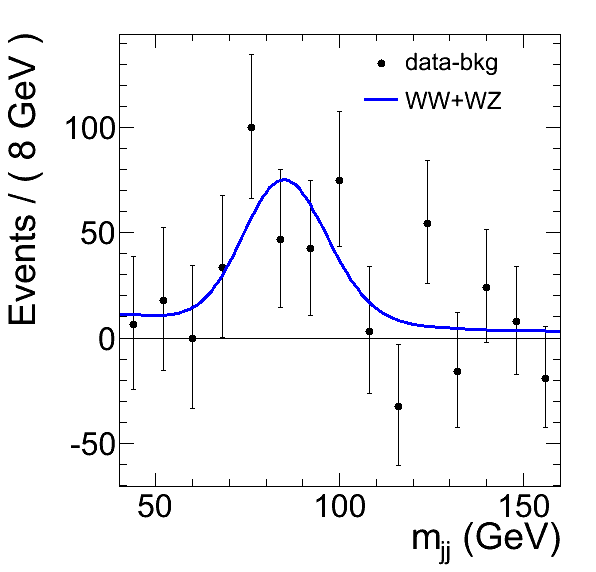
\includegraphics[width=0.49\textwidth]{figs/mjjfit/DibosonBtaglnujj_muon_Subtracted.png}
    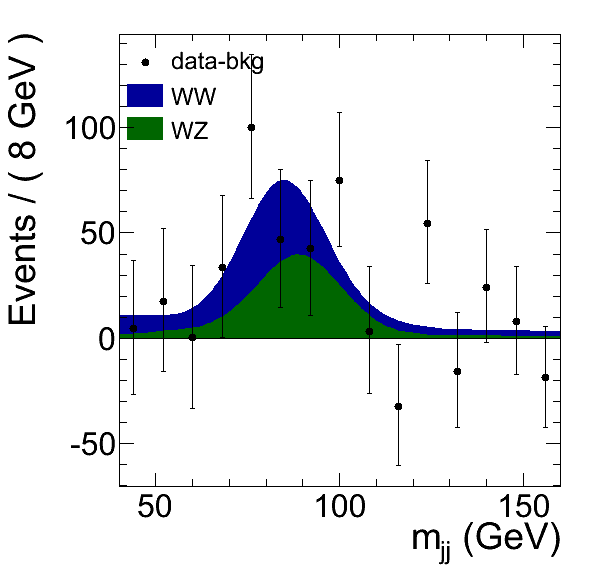
\includegraphics[width=0.49\textwidth]{figs/mjjfit/DibosonBtaglnujj_muon_Split.png}
    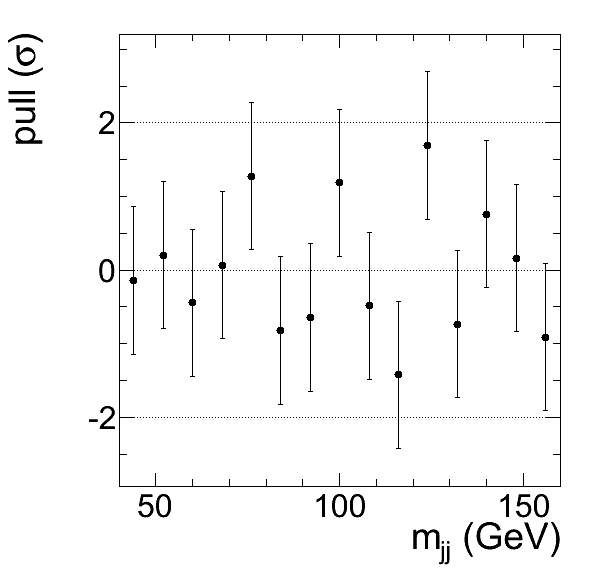
\includegraphics[width=0.49\textwidth]{figs/mjjfit/DibosonBtaglnujj_muon_Pull.png}
    \caption{Distribution of the dijet invariant mass for the (non-boosted) btagged 2-jet events in muon data and fit shapes: 
      (upper left) All background components stacked together, 
      (upper right) Data minus all backgrounds except diboson,
      (lower left) Data minus all backgrounds except diboson with $WW$ and $WZ$ contributions shown separately,
      (lower right) normalized residual between data and MC. The vertical dotted lines
      indicate the mass intbrval excluded from the fit.}
    \label{fig:mjj_2jet_mu_btag}}
\end{figure}
%%%%%%%%%%%%%%%%%%%%%
%%%%%%%%%%%%%%%%%%%%%
\begin{figure}[h!]
  {\centering
    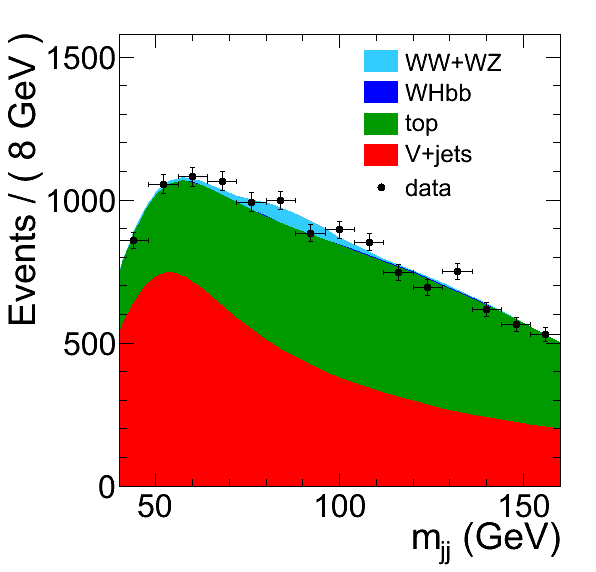
\includegraphics[width=0.49\textwidth]{figs/mjjfit/DibosonBtaglnujj_electron_Stacked.png}
    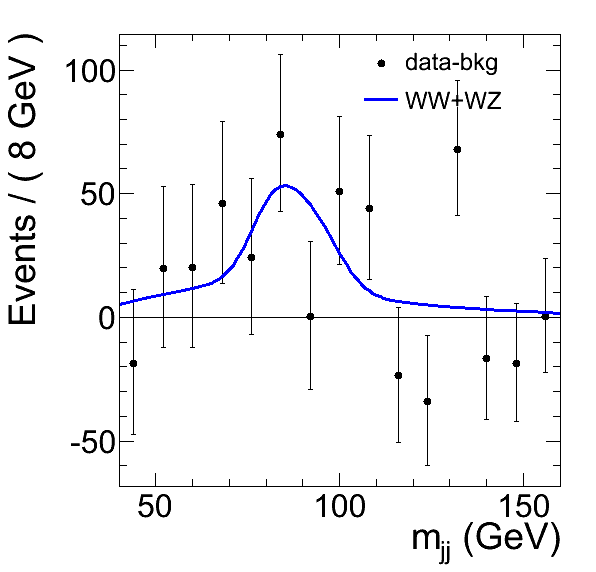
\includegraphics[width=0.49\textwidth]{figs/mjjfit/DibosonBtaglnujj_electron_Subtracted.png}
    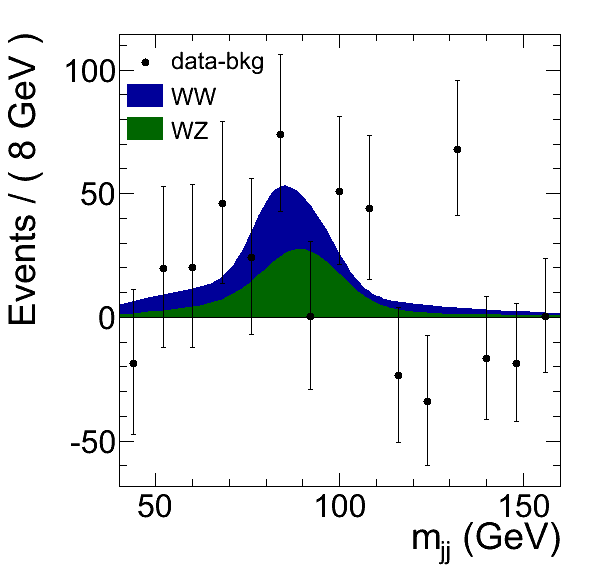
\includegraphics[width=0.49\textwidth]{figs/mjjfit/DibosonBtaglnujj_electron_Split.png}
    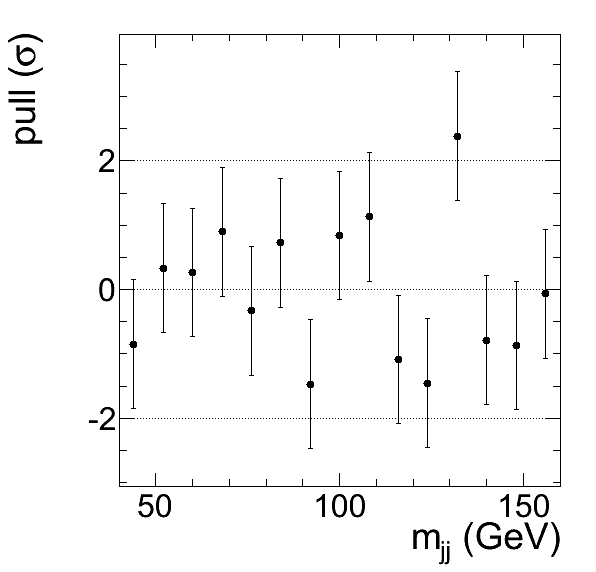
\includegraphics[width=0.49\textwidth]{figs/mjjfit/DibosonBtaglnujj_electron_Pull.png}
    \caption{Distribution of the dijet invariant mass for the (non-boosted) btagged 2-jet events in electron data and fit shapes: 
      (upper left) All background components stacked together, 
      (upper right) Data minus all backgrounds except diboson,
      (lower left) Data minus all backgrounds except diboson with $WW$ and $WZ$ contributions shown separately,
      (lower right) normalized residual between data and MC. The vertical dotted lines
      indicate the mass interval excluded from the fit.}
    \label{fig:mjj_2jet_el_btag}}
\end{figure}
%%%%%%%%%%%%%%%%%%%%%
%%%%%%%%%%%%%%%%%%%%
\begin{figure}[h!]
  {\centering
    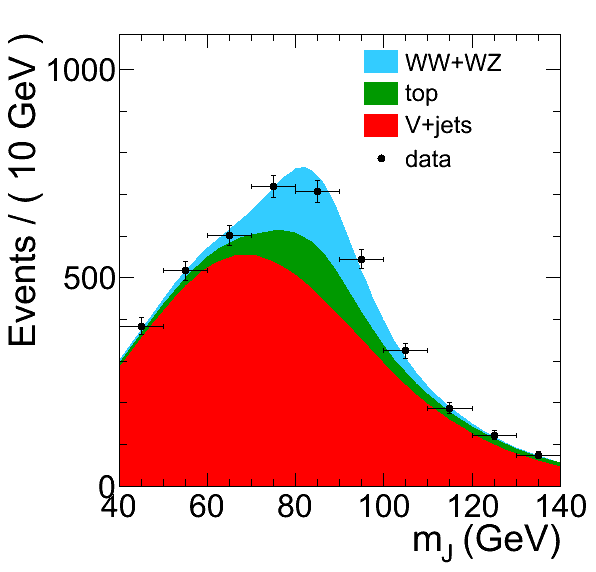
\includegraphics[width=0.49\textwidth]{figs/mjjfit/DibosonBoostedlnuJ_muon_Stacked.png}
    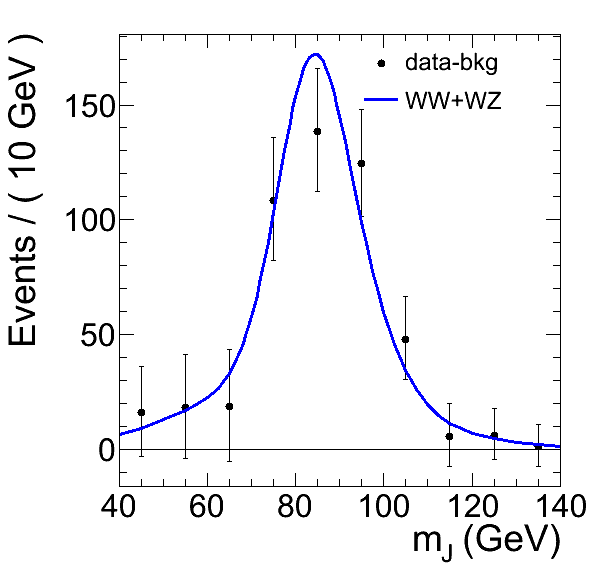
\includegraphics[width=0.49\textwidth]{figs/mjjfit/DibosonBoostedlnuJ_muon_Subtracted.png}
    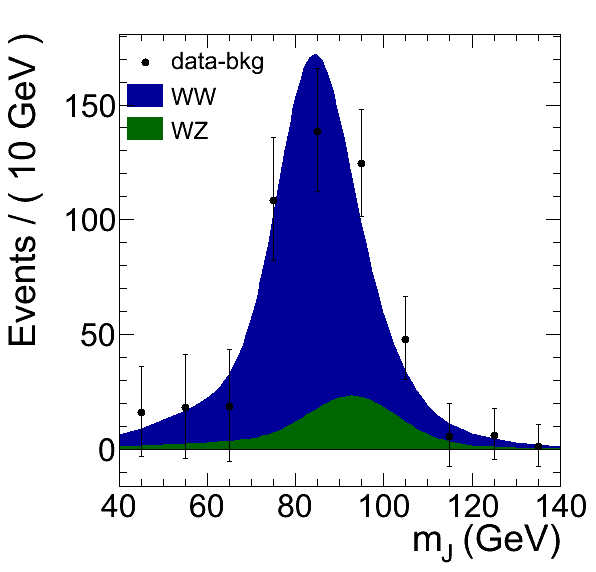
\includegraphics[width=0.49\textwidth]{figs/mjjfit/DibosonBoostedlnuJ_muon_Split.png}
    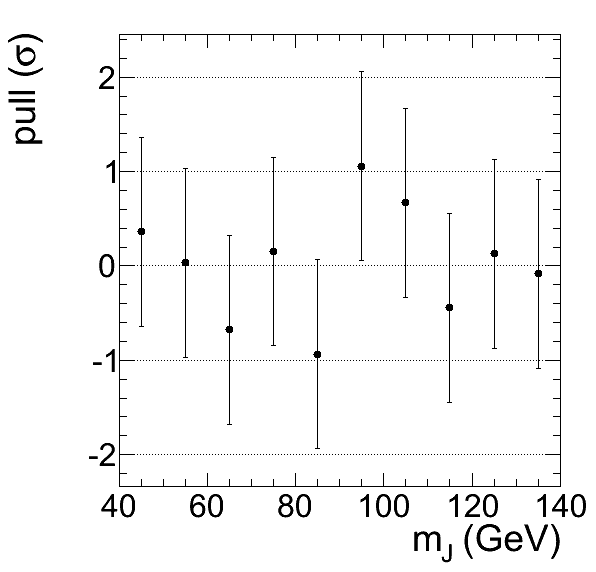
\includegraphics[width=0.49\textwidth]{figs/mjjfit/DibosonBoostedlnuJ_muon_Pull.png}
    \caption{Distribution of the W-jet invariant mass for the boosted events in muon data and fit shapes: 
      (upper left) All background components stacked together, 
      (upper right) Data minus all backgrounds except diboson,
      (lower left) Data minus all backgrounds except diboson with $WW$ and $WZ$ contributions shown separately,
      (lower right) normalized residual between data and MC. The vertical dotted lines
      indicate the mass interval excluded from the fit.}
    \label{fig:mJ_mu_boosted}}
\end{figure}
%%%%%%%%%%%%%%%%%%%%
%%%%%%%%%%%%%%%%%%%%
\begin{figure}[h!]
  {\centering
    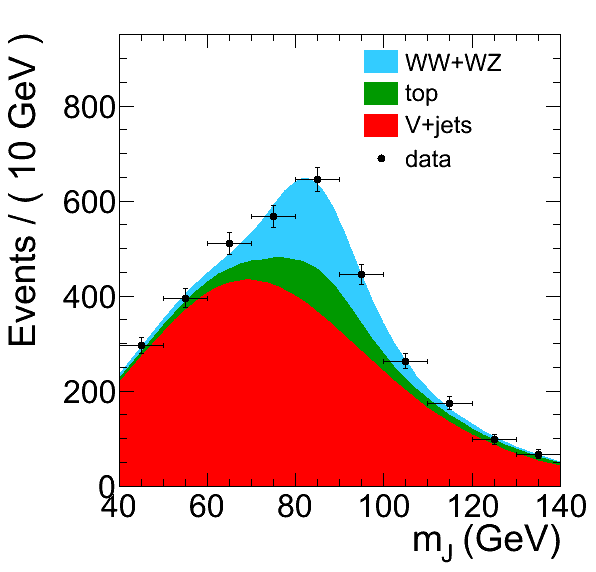
\includegraphics[width=0.49\textwidth]{figs/mjjfit/DibosonBoostedlnuJ_electron_Stacked.png}
    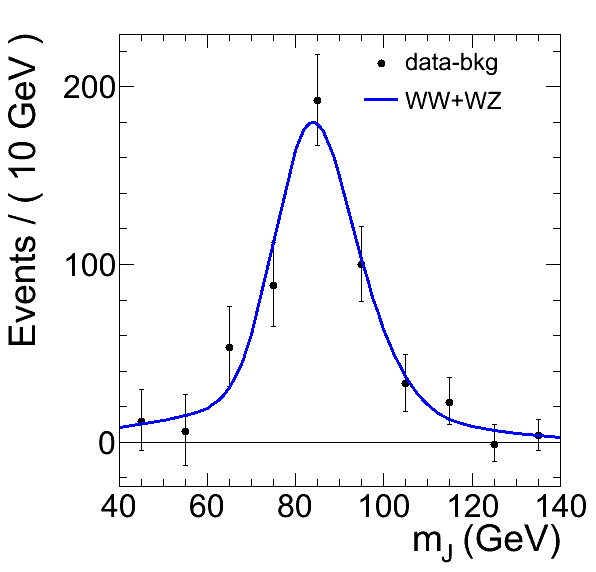
\includegraphics[width=0.49\textwidth]{figs/mjjfit/DibosonBoostedlnuJ_electron_Subtracted.png}
    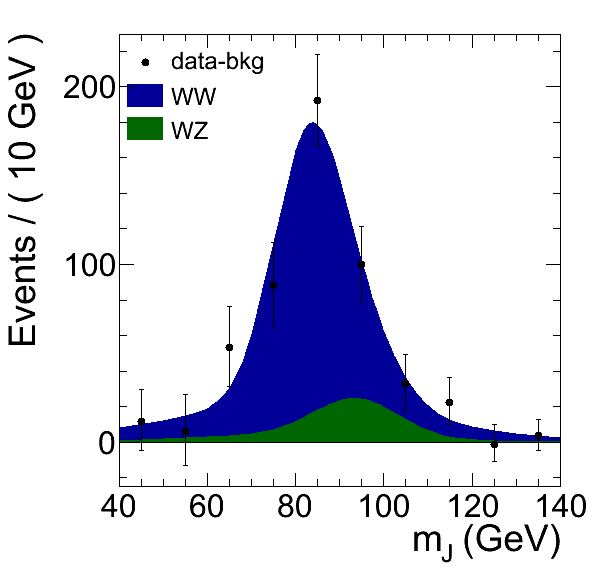
\includegraphics[width=0.49\textwidth]{figs/mjjfit/DibosonBoostedlnuJ_electron_Split.png}
    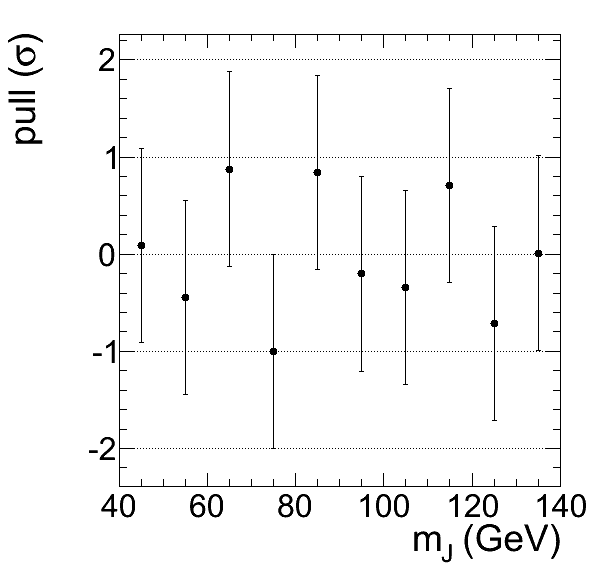
\includegraphics[width=0.49\textwidth]{figs/mjjfit/DibosonBoostedlnuJ_electron_Pull.png}
    \caption{Distribution of the W-jet invariant mass for the boosted events in electron data and fit shapes: 
      (upper left) All background components stacked together, 
      (upper right) Data minus all backgrounds except diboson,
      (lower left) Data minus all backgrounds except diboson with $WW$ and $WZ$ contributions shown separately,
      (lower right) normalized residual between data and MC. The vertical dotted lines
      indicate the mass interval excluded from the fit.}
    \label{fig:mJ_el_boosted}}
\end{figure}
%%%%%%%%%%%%%%%%%%%%
%%%%%%%%%%%%%%%%%%%%
%%%%%%%%%%%%%%%
%%%%%%%%%%%%%%%
\begin{table}[tbht!]
\begin{center}
\caption{Fractions of the expected yields (or the total yield) determined from a likelihood fit to the data, the expected event counts and the Diboson Fraction as well as Error corrected for the fit bias (as described in Section~\ref{sec:FitValidation}.}
 \label{table:FitTotalsAndComparisons}
\vspace{0.5cm}
 \begin{tabular} {l  c  c c c }
   \hline \hline
Bin            &  \multicolumn{2}{c}{muons, anti-btagged dijet} & \multicolumn{2}{c}{electrons, anti-btagged dijet} \\  
\hline
               & Predicted &   Extracted Fraction     &  Predicted &  Extracted Fraction \\
\hline
Diboson        & 2640 & 1.43$\pm$0.28   &   2300 & 1.73$\pm$0.32 \\
Multijet       &  ---   &   ---              & 8520     &   1.18$\pm$0.36  \\
Top            & 4272   &   1.00$\pm$0.07  & 3620     &   1.00$\pm$0.07  \\
V+Jets         & 117079 &   1.01$\pm$0.01  & 101330   &   1.03$\pm$0.03  \\
Total Yields   & 123991 &   126759         & 115770   &   121698  \\ 
\hline 
Corrected Diboson & 2640 & 1.49$\pm$0.28   &   2300 & 1.65$\pm$0.29 \\
\hline 
Data           & 126760 & ---        & 121709 & ---   \\ 
\hline
\\
\hline
\hline
Bin             &  \multicolumn{2}{c}{muons,btagged dijet} & \multicolumn{2}{c}{electrons, btagged dijet} \\  
\hline
                & Predicted &   Extracted Fraction     &  Predicted &  Extracted Fraction \\
\hline
Diboson         & 193 & 1.81$\pm$0.68   &   163 & 1.45$\pm$0.80 \\
Top             & 7011     &   0.99$\pm$0.03  & 5959    &   0.99$\pm$0.04  \\
V+Jets          & 6774     &   0.99$\pm$0.03  & 6437    &   1.00$\pm$0.04  \\
$WH(150)\to bb$ & 23       &   1.0              & 20      &   1.0 \\
Total Yields    & 14001    &   14007            & 12579   &   12588  \\ 
\hline 
Corrected Diboson & 193 & 1.72$\pm$0.64   &   163 & 1.25$\pm$0.70  \\
\hline 
Data            & 14001 & ---        & 12586 & ---  \\
\hline 
\\
\hline
\hline
Bin            &  \multicolumn{2}{c}{muons,  boosted} & \multicolumn{2}{c}{electrons, boosted} \\  
\hline
               & Predicted &   Extracted Fraction     &  Predicted &  Extracted Fraction \\
\hline
Diboson        & 245       & 1.99$\pm$1.03            &   218 & 2.33$\pm$0.56 \\
Top            & 396       &   1.00$\pm$0.08  & 322     &   1.00$\pm$0.10  \\
V+Jets         & 3269      &   1.01$\pm$0.08  & 2769     &   0.95$\pm$0.05  \\
Total Yields   & 3910      &   4182           & 3309     &   3461  \\ 
\hline 
Corrected Diboson & 245 & 1.86$\pm$1.13   &   218 & 2.27$\pm$0.67 \\
\hline
Data & 4181 & ---        & 3461 & --- \\  
\hline
\hline
\end{tabular}
\end{center}
\end{table}

\begin{table}[bthp]
\begin{center}
\caption{\label{tab:dibosonYield} Diboson signal yields along with corresponding cross-sections, with the statistical contribution and the systematic contribution to the uncertainties broken out. The first uncertainty arises chiefly from statistics the second is from systematic sources.}
\begin{tabular}{rcc}
\hline\hline
& muons, anti-btagged & electrons, anti-btagged \\
\hline
N Diboson             & 3942$\pm$356$\pm$650   &   3804$\pm$349$\pm$571   \\
$\sigma_{WW+WZ}$(pb)    & 119.47$\pm$10.79$\pm$19.70   &   133.20$\pm$12.22$\pm$19.99   \\
\hline
& muons, btagged & electrons, btagged \\
\hline
N Diboson             & 331$\pm$118$\pm$35   &   204$\pm$112$\pm$22   \\
$\sigma_{WW+WZ}$(pb)    & 137.41$\pm$49.05$\pm$14.53   &   100.20$\pm$55.22$\pm$10.62   \\
\hline
& muons, boosted & electrons, boosted \\
\hline
N Diboson & 456$\pm$65$\pm$269   &   497$\pm$59$\pm$133 \\
$\sigma_{WW+WZ}$(pb) & 111.50$\pm$15.81$\pm$65.73   &   139.30$\pm$16.50$\pm$37.44 \\
\hline\hline
\end{tabular}
\end{center}
\end{table}
%%%%%%%%%%%%%%%
%%%%%%%%%%%%%%%
%%%%%%%%%%%%%%%%%%%%%%%%%%%%%%%%%%%%%%%%%%%%%%%%%%%%%%%%%%%%

%%%%%%%%%%%%%%%
\begin{table}[bthp]
\begin{center}
\caption{\label{tab:SystematicCorrections} Diboson extracted yield, significance and corresponding fit systematics for each channel. The Yield is corrected for the bias, while the error is inflated by the fractional error bias with the shape systematic added in quadrature.}
\begin{tabular}{rcc}
\hline\hline
Quantity       & muons, anti-btagged & electrons, anti-btagged \\
\hline
Fit Yield      & 3942$\pm$741   &   3804$\pm$669 \\
Significance   & $4.9\sigma$	     & $5.2\sigma$  \\
Yield Bias     & -161                & +164   \\
Fractional Error Bias     & 0.89		     & 0.90   \\
Shape Systematic & 320		     & 107   \\
\hline
& muons, btagged & electrons, btagged \\
\hline
Fit Yield      & 331$\pm$123   &   204$\pm$114 \\
Significance   & $3.3\sigma$       & $1.5\sigma$  \\
Yield Bias     & +17		   & +33   \\
Fractional Error Bias     & 0.94		   & 0.83   \\
Shape Systematic & 6		   & 38   \\
\hline
& muons, boosted & electrons, boosted \\
\hline
Fit Yield & 456$\pm$277   &   497$\pm$146 \\
Significance   & $3.5\sigma$       & $3.9\sigma$   \\
Yield Bias     & +31.4		   & +12.3   \\
Fractional Error Bias     & 0.96		   & 0.98   \\
Shape Systematic & 133		   & 83     \\
\hline\hline
\end{tabular}
\end{center}
\end{table}
%%%%%%%%%%%%%%%



%%%%%%%%%%%%%%%%%%%%%%%%%%%%%%%%%%%%%%%%%%%%%%%%%%%%%%%%%%%%
%%%%%%%%%%%%%%%%%%%%%%%%%%%%%%%%%%%%%%%%%%%%%%%%%%%%%%%%%%%%
\clearpage
\subsection{Fit Validation}
\label{sec:FitValidation}
We verify that the signal extraction procedure is unbiased and that 
statistical uncertainties reported have good coverage by constructing
and fitting toy datasets. Since our fit procedure is the same in both
electron and muon channels, we validate and perform a number of cross-checks
using muons; with the electron results subsequently listed. 
The specific steps are:
\begin{enumerate}
\item Perform the default fit and obtain the expected yields 
(Table~\ref{table:FitTotalsAndComparisons}).
\item Generate toy Monte Carlo for each process from the corresponding MC distributions.
\item Construct 1000 sample datasets. The excpected yield are first smeared by the fit 
errors, with correlations taken into account, by computing the errors in a coordinate frame 
where they are uncorrelated and rotating back (Sec.~\ref{sec:FitValidation_ExpectedEventGeneration}). 
Afterwards, we smear the expected yields by the Poisson Errors.
\item Perform the fit for each sample dataset.
\item Examine the resultant Yields and Pulls.
\end{enumerate}


\subsubsection{Expected Event Generation}
\label{sec:FitValidation_ExpectedEventGeneration}
Due to the constraints imposed by the data, the fitted event yields are strongly correlated
(Sec.~\ref{sec:mjj_2jetfit}). This fact is taken into account 
when smearing the expected values. In short we perform a transformation to 
the coordinate system where the yields are uncorrelated, smear and transform back. Specifically,
for each toy dataset we:
\begin{enumerate}
\item Diagonalize the Covariance Matrix ($\Sigma$) obtained from the original fit to the 
data (Sec.~\ref{sec:mjj_2jetfit}). I.e. find $M$ such that $M\Sigma M^{-1}$ is 
diagonal (Rows of $M$ are in fact the eigenvectors of $\Sigma$).
\item Produce the errors ($z_i$) in a frame where there is no correlation between the fitted 
'yields' (i.e. in a frame where the Covariance Matrix is diagonal). Namely, $z_i$ are randomly 
selected from a Gaussian distribution with $\sigma_i^2=(M\Sigma M^{-1})_{ii}$ and mean$=0$.
\item Transform back to the orignal frame and obtain the yields ($x_i$) smeared by the fit error: 
$x_i=\mu_i+(M^{-1}Z)_i$, where $\mu$ is the expected value from the default fit.
\item Poisson-smear $x_i$ and generate the dataset with the obtained values.
\item Perform the fit.
\end{enumerate}
This procedure is designed to sample in the vicinity of the fit result, while taking the likelihood of a particular configuration into account. The resultant Yield and Pull distributions are examined to see if they are Gaussian, whether there is any bias in the yield and how close the pull $\sigma$ is to unity.


\subsubsection{Fit Configuration Validation}
The first step is to determine if there is any inherent bias in the fit. As such we use the yield and shape parameter values returned by the fit to generate toy datasets and refit them.
The results are shown in Figs.~\ref{fig:Validation_mu_Standard},~\ref{fig:Validation_el_Standard} for the anti-btagged dijet configuration, Figs.~\ref{fig:Validation_mu_Btag},~\ref{fig:Validation_el_Btag} for the btagged dijet configuration and in Figs.~\ref{fig:Validation_mu_Boosted},~\ref{fig:Validation_el_Boosted} for the boosted case.

%%%%%%%%%%%%%%%%%%%%%%%%%
%%%%%%%
\begin{figure}[h!] {\centering
\unitlength=0.33\linewidth
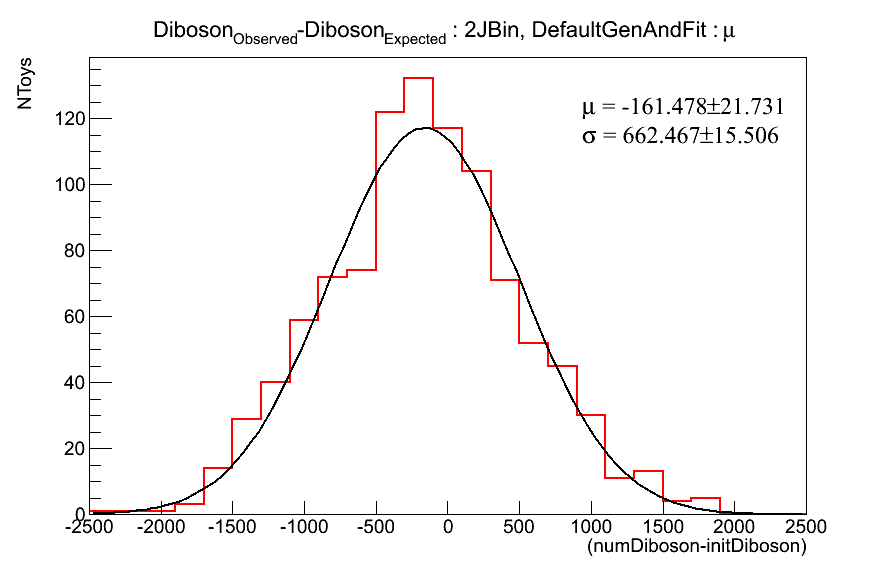
\includegraphics[width=0.48\textwidth]{figs/validation/Validation_DibosonYield_Standard_mu.png}
\put(-0.80,0.0){(a)}
\unitlength=0.33\linewidth
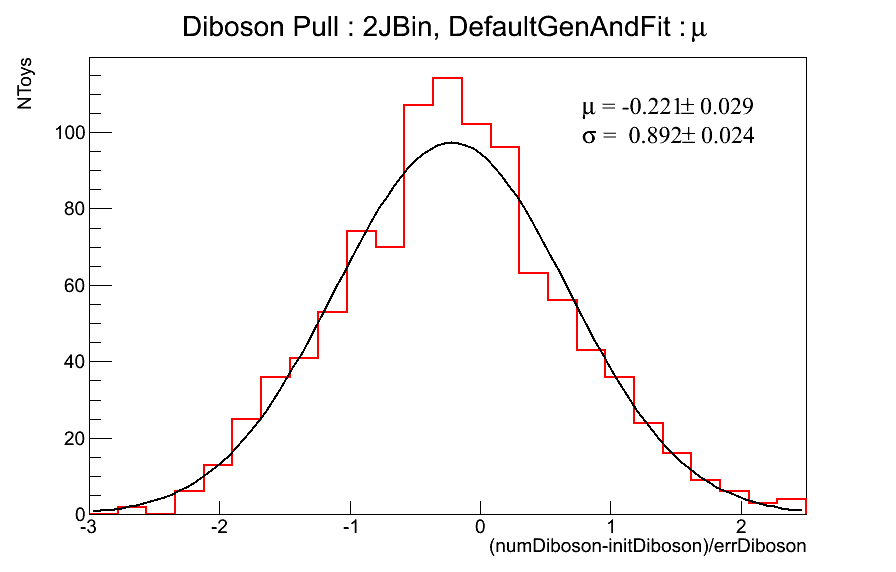
\includegraphics[width=0.48\textwidth]{figs/validation/Validation_DibosonPull_Standard_mu.png}
\put(-0.80,0.0){(b)} \\ 
\unitlength=0.33\linewidth
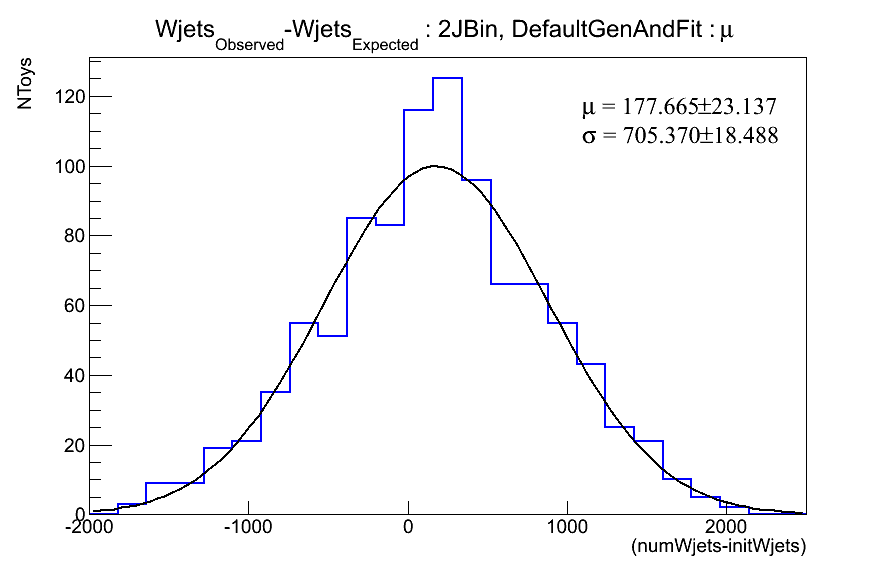
\includegraphics[width=0.48\textwidth]{figs/validation/Validation_WJetsYield_Standard_mu.png}
\put(-0.80,0.0){(c)}
\unitlength=0.33\linewidth
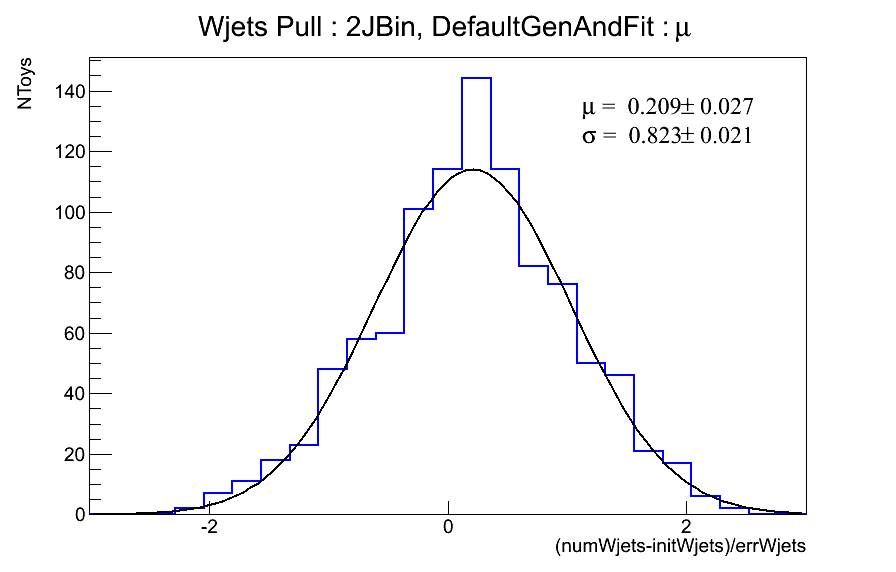
\includegraphics[width=0.48\textwidth]{figs/validation/Validation_WJetsPull_Standard_mu.png}
\put(-0.80,0.0){(d)} 
\caption{Fit validation in the (anti-btagged) dijet the muon channel, using 1000 Toy MC datasets. Fitted-Given yields for: (a) Diboson, (c) V+Jets and Pull=(Fitted-Given)/Error for: (b) Diboson, (d) V+Jets.} 
\label{fig:Validation_mu_Standard}}
\end{figure}
%%%%%%%
%%%%%%%
\begin{figure}[h!] {\centering
\unitlength=0.33\linewidth
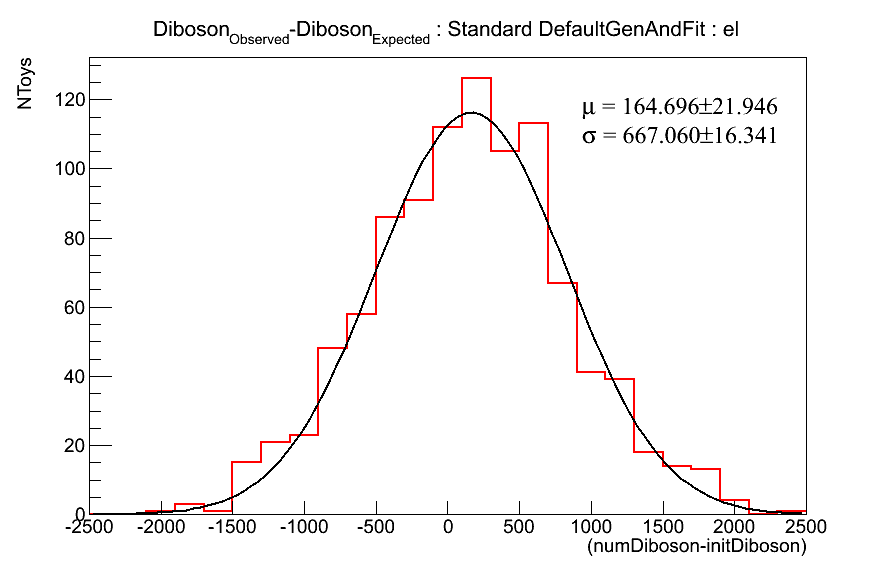
\includegraphics[width=0.48\textwidth]{figs/validation/Validation_DibosonYield_Standard_el.png}
\put(-0.80,0.0){(a)}
\unitlength=0.33\linewidth
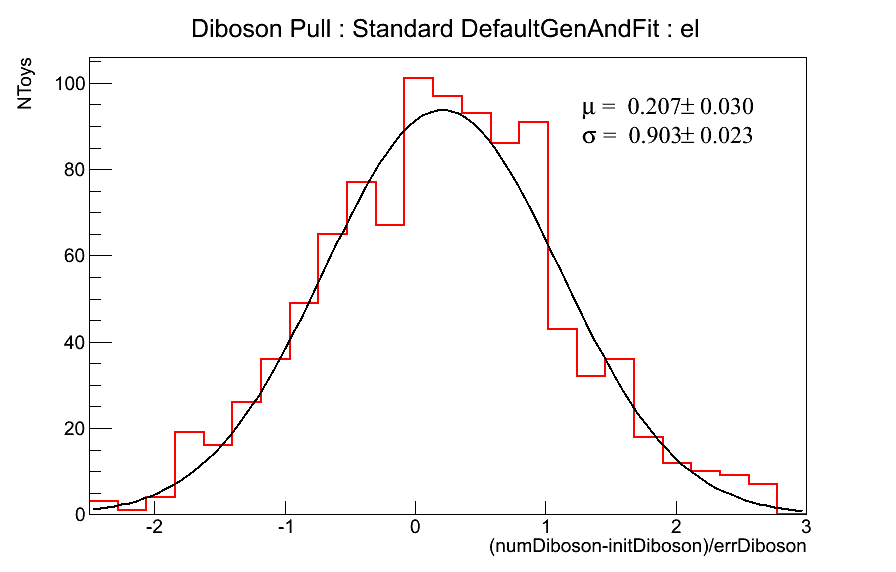
\includegraphics[width=0.48\textwidth]{figs/validation/Validation_DibosonPull_Standard_el.png}
\put(-0.80,0.0){(b)} \\ 
\unitlength=0.33\linewidth
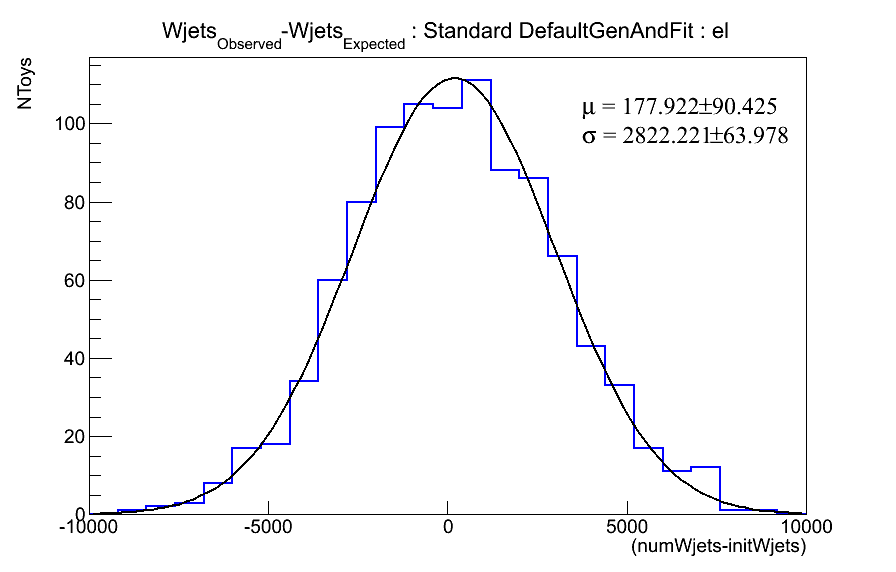
\includegraphics[width=0.48\textwidth]{figs/validation/Validation_WJetsYield_Standard_el.png}
\put(-0.80,0.0){(c)}
\unitlength=0.33\linewidth
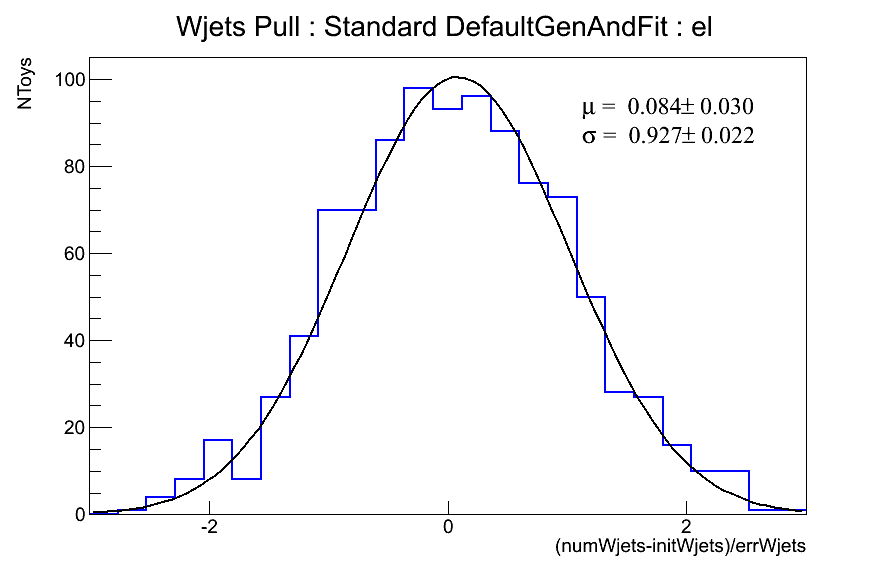
\includegraphics[width=0.48\textwidth]{figs/validation/Validation_WJetsPull_Standard_el.png}
\put(-0.80,0.0){(d)} 
\caption{Fit validation in the (anti-btagged) dijet the electron channel, using 1000 Toy MC datasets. Fitted-Given yields for: (a) Diboson, (c) V+Jets and Pull=(Fitted-Given)/Error for: (b) Diboson, (d) V+Jets.} 
\label{fig:Validation_el_Standard}}
\end{figure}
%%%%%%%
%%%%%%%
\begin{figure}[h!] {\centering
\unitlength=0.33\linewidth
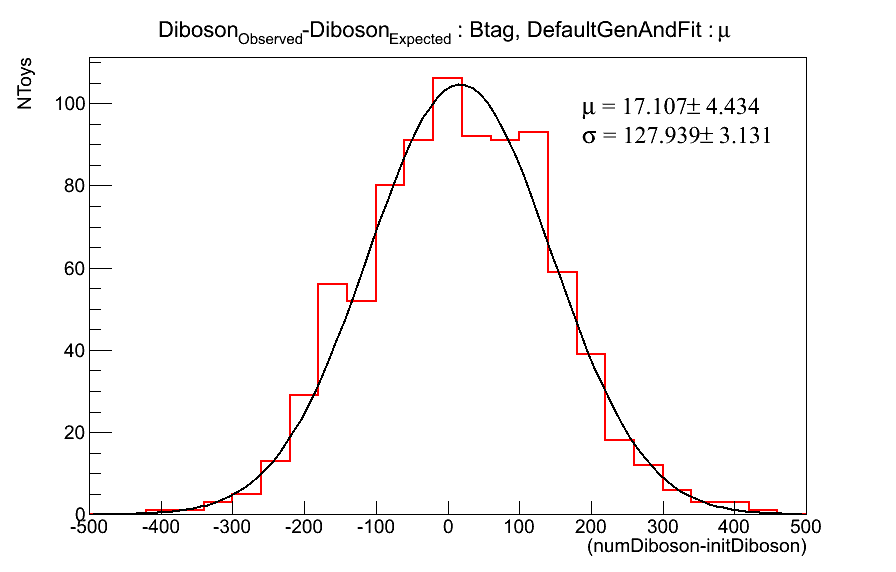
\includegraphics[width=0.48\textwidth]{figs/validation/Validation_DibosonYield_Btag_mu.png}
\put(-0.80,0.0){(a)}
\unitlength=0.33\linewidth
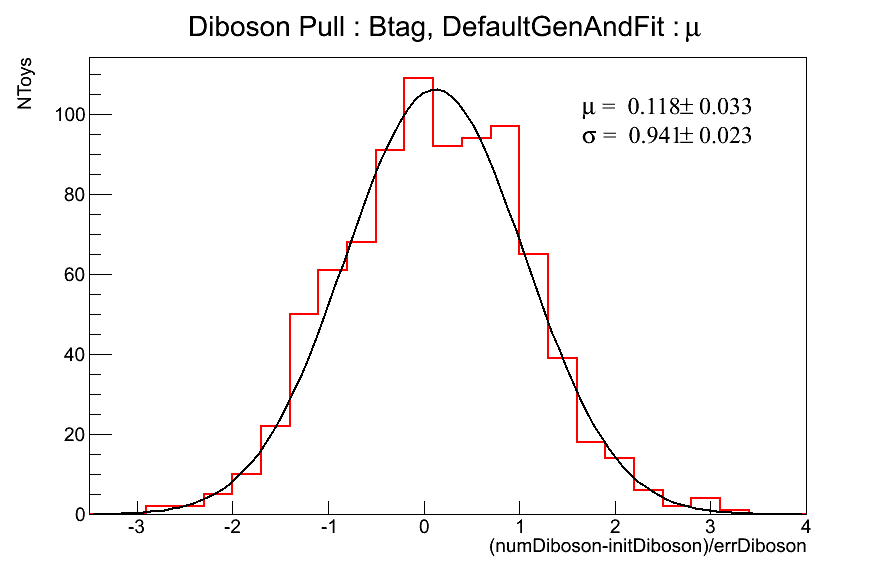
\includegraphics[width=0.48\textwidth]{figs/validation/Validation_DibosonPull_Btag_mu.png}
\put(-0.80,0.0){(b)} \\ 
\unitlength=0.33\linewidth
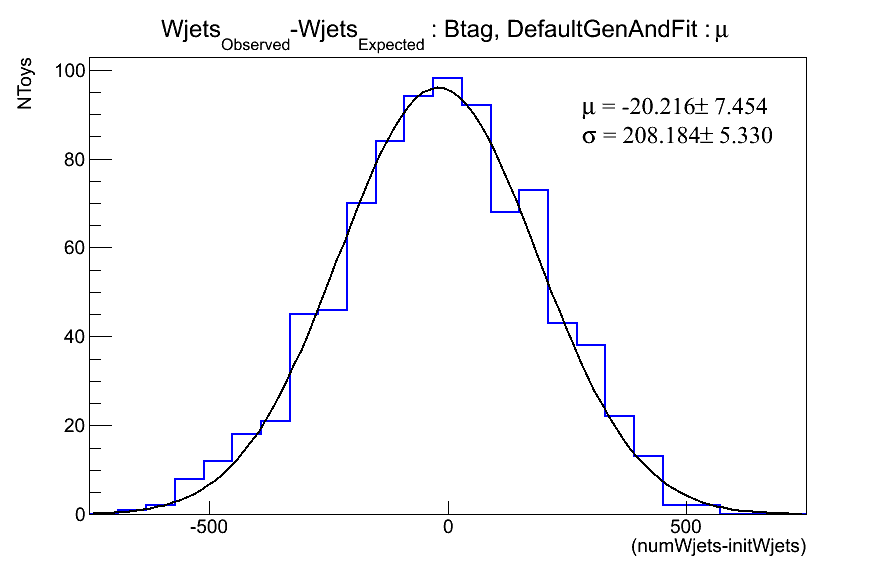
\includegraphics[width=0.48\textwidth]{figs/validation/Validation_WJetsYield_Btag_mu.png}
\put(-0.80,0.0){(c)}
\unitlength=0.33\linewidth
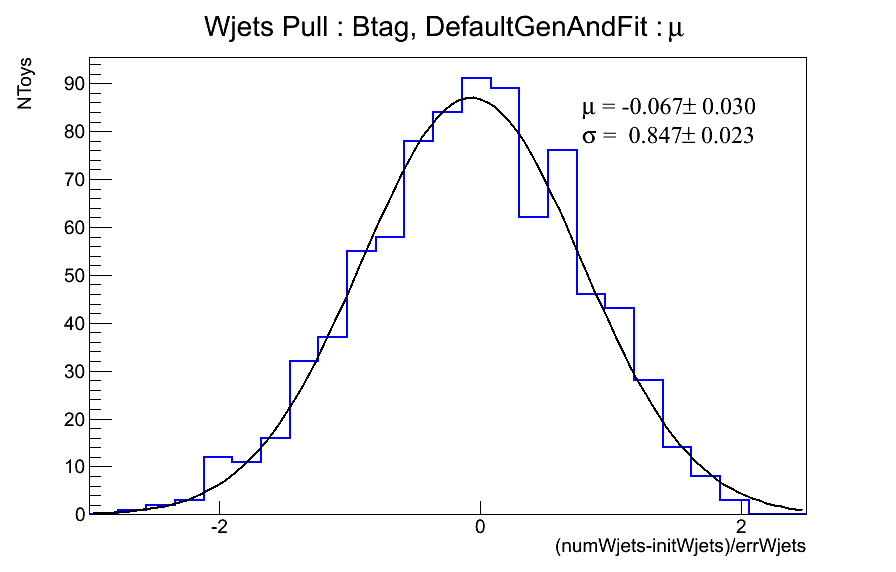
\includegraphics[width=0.48\textwidth]{figs/validation/Validation_WJetsPull_Btag_mu.png}
\put(-0.80,0.0){(d)} \\
\unitlength=0.33\linewidth
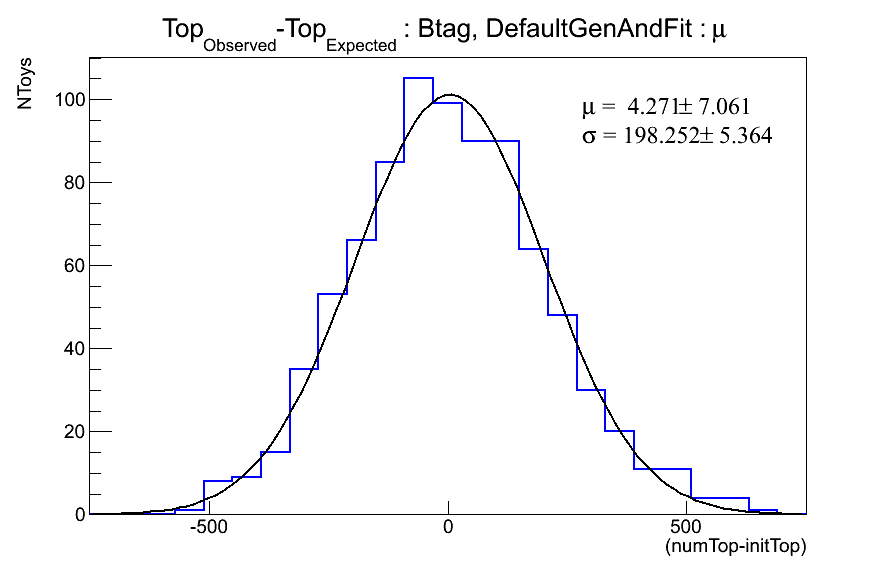
\includegraphics[width=0.48\textwidth]{figs/validation/Validation_topYield_Btag_mu.png}
\put(-0.80,0.0){(e)}
\unitlength=0.33\linewidth
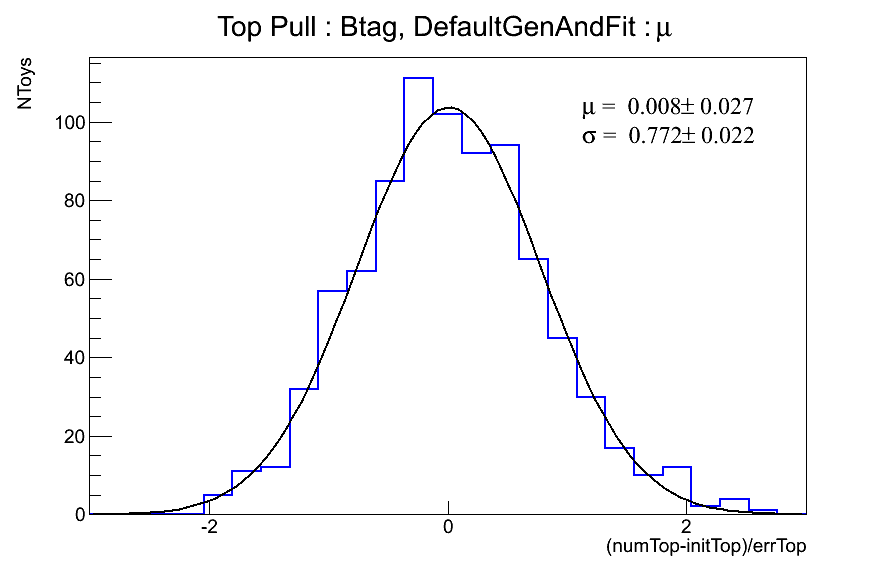
\includegraphics[width=0.48\textwidth]{figs/validation/Validation_topPull_Btag_mu.png}
\put(-0.80,0.0){(f)} 
\caption{Fit validation in the btagged dijet the muon channel, using 1000 Toy MC datasets. Fitted-Given yields for: (a) Diboson, (c) V+Jets, (e) top and Pull=(Fitted-Given)/Error for: (b) Diboson, (d) V+Jets, (f) top.} 
\label{fig:Validation_mu_Btag}}
\end{figure}
%%%%%%%
%%%%%%%
\begin{figure}[h!] {\centering
\unitlength=0.33\linewidth
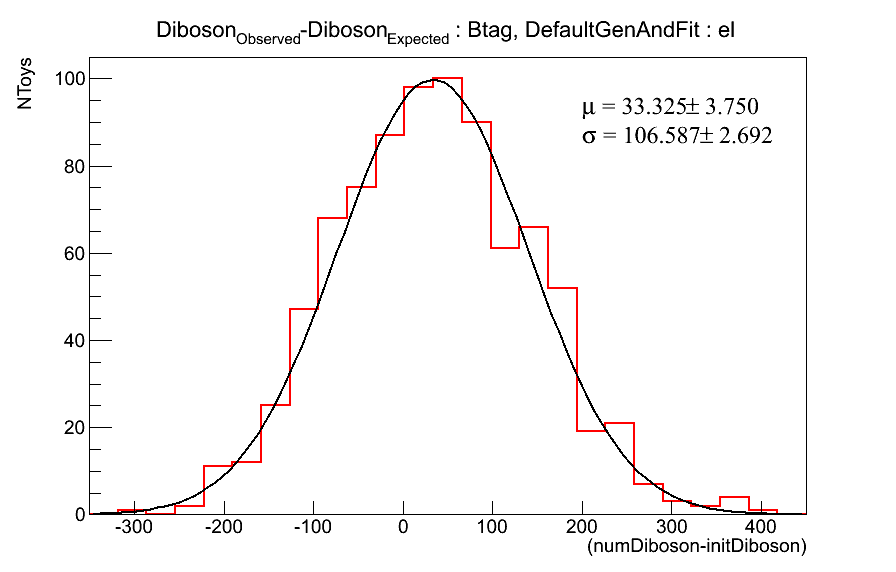
\includegraphics[width=0.48\textwidth]{figs/validation/Validation_DibosonYield_Btag_el.png}
\put(-0.80,0.0){(a)}
\unitlength=0.33\linewidth
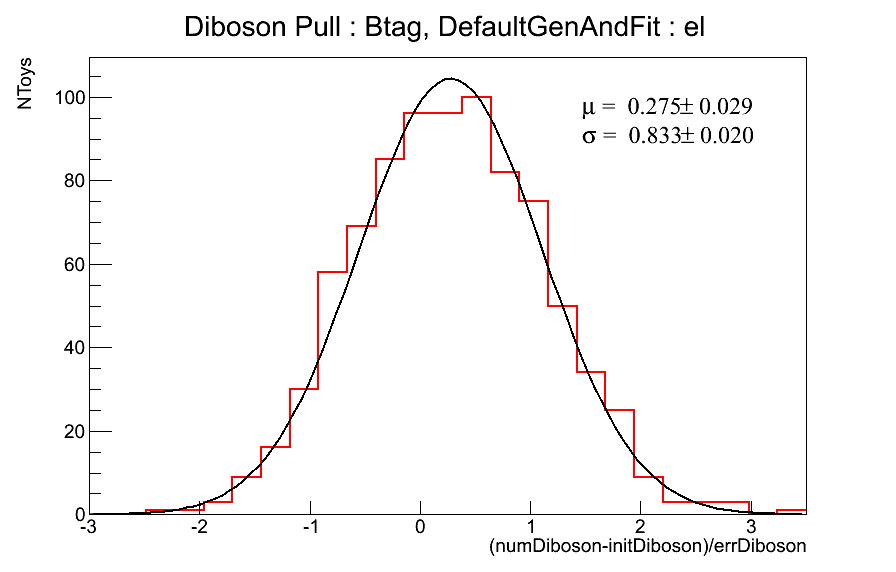
\includegraphics[width=0.48\textwidth]{figs/validation/Validation_DibosonPull_Btag_el.png}
\put(-0.80,0.0){(b)} \\ 
\unitlength=0.33\linewidth
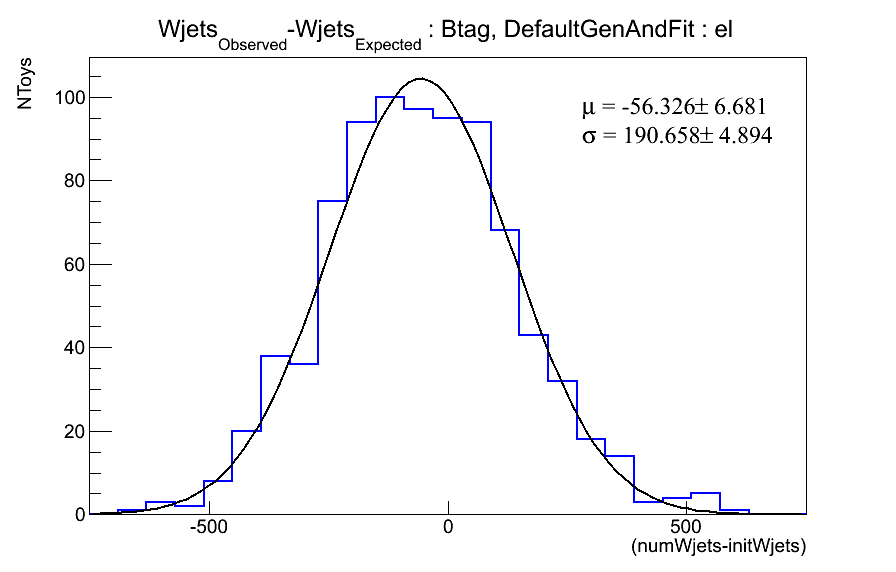
\includegraphics[width=0.48\textwidth]{figs/validation/Validation_WJetsYield_Btag_el.png}
\put(-0.80,0.0){(c)}
\unitlength=0.33\linewidth
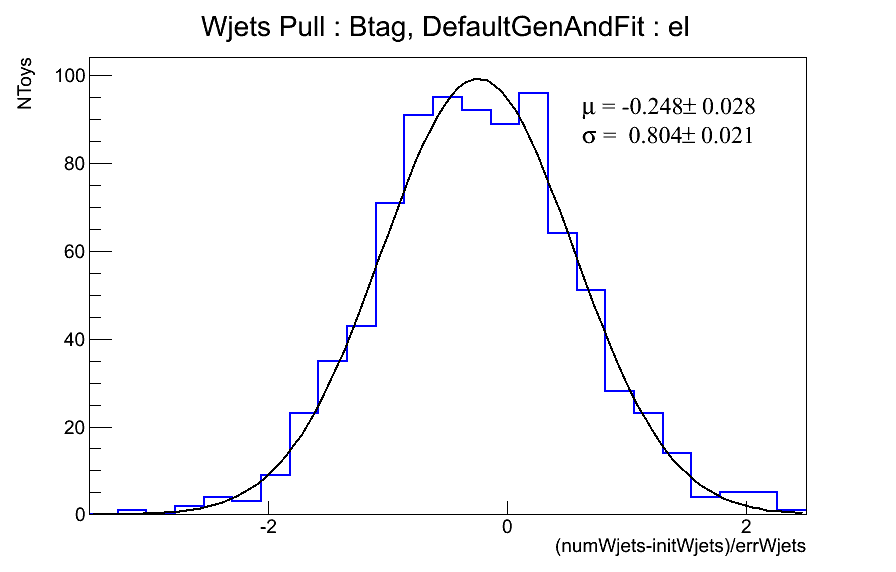
\includegraphics[width=0.48\textwidth]{figs/validation/Validation_WJetsPull_Btag_el.png}
\put(-0.80,0.0){(d)} \\
\unitlength=0.33\linewidth
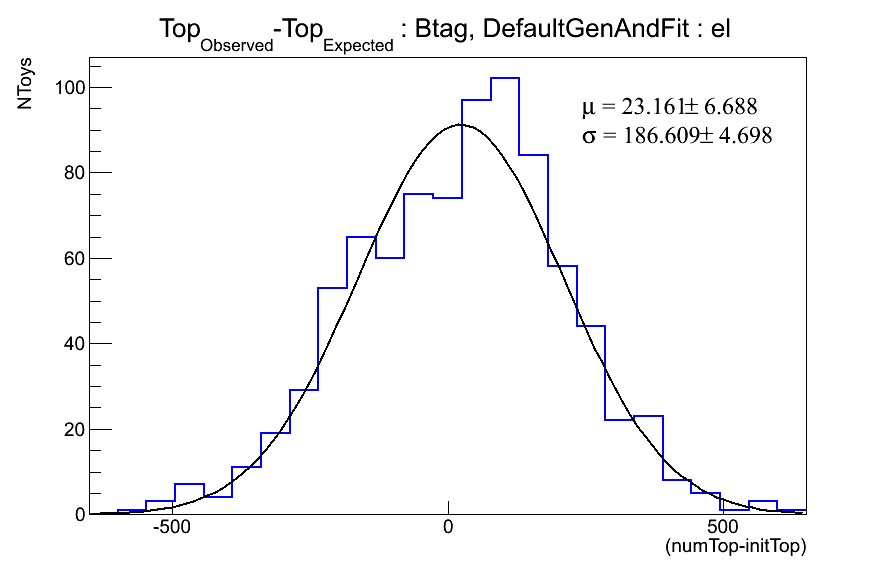
\includegraphics[width=0.48\textwidth]{figs/validation/Validation_topYield_Btag_el.png}
\put(-0.80,0.0){(e)}
\unitlength=0.33\linewidth
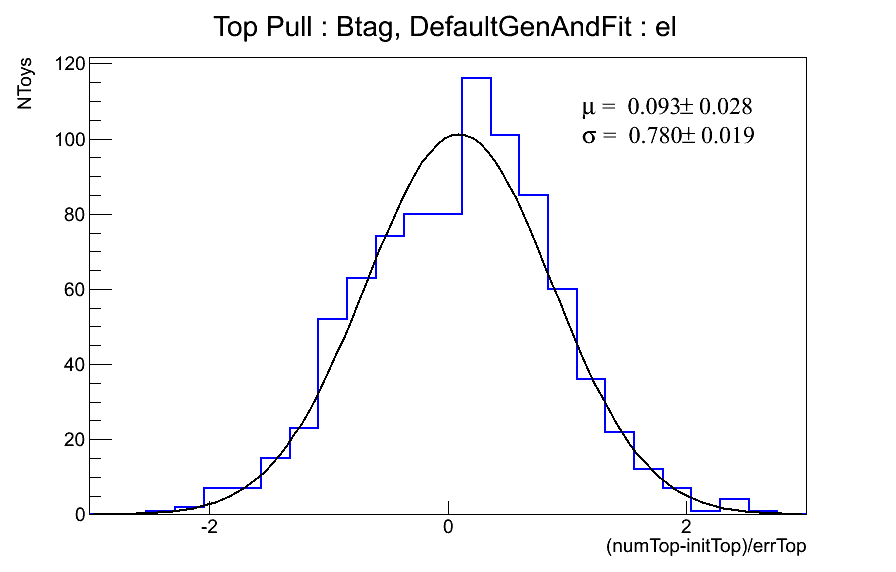
\includegraphics[width=0.48\textwidth]{figs/validation/Validation_topPull_Btag_el.png}
\put(-0.80,0.0){(f)} 
\caption{Fit validation in the btagged dijet the electron channel, using 1000 Toy MC datasets. Fitted-Given yields for: (a) Diboson, (c) V+Jets, (e) top and Pull=(Fitted-Given)/Error for: (b) Diboson, (d) V+Jets, (f) top.} 
\label{fig:Validation_el_Btag}}
\end{figure}
%%%%%%%
%%%%%%%
\begin{figure}[h!] {\centering
\unitlength=0.33\linewidth
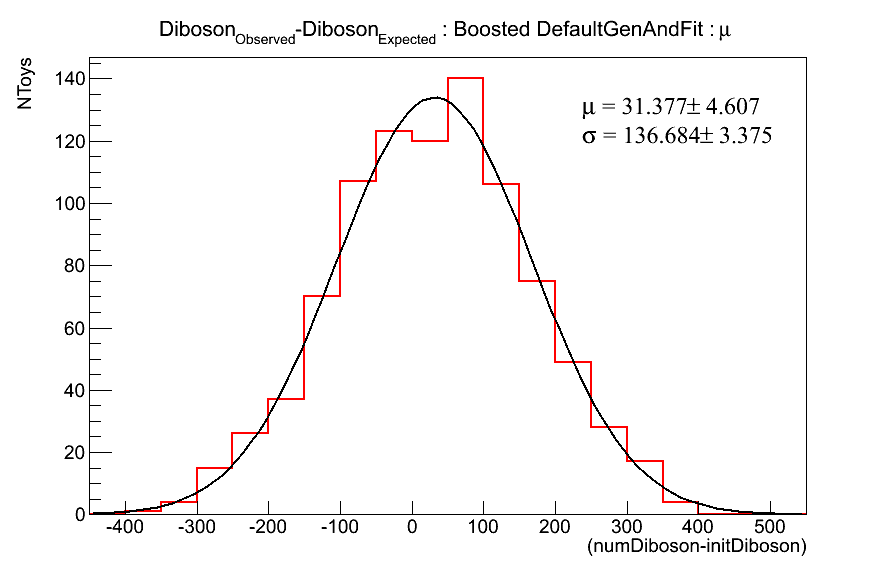
\includegraphics[width=0.48\textwidth]{figs/validation/Validation_DibosonYield_Boosted_mu.png}
\put(-0.80,0.0){(a)}
\unitlength=0.33\linewidth
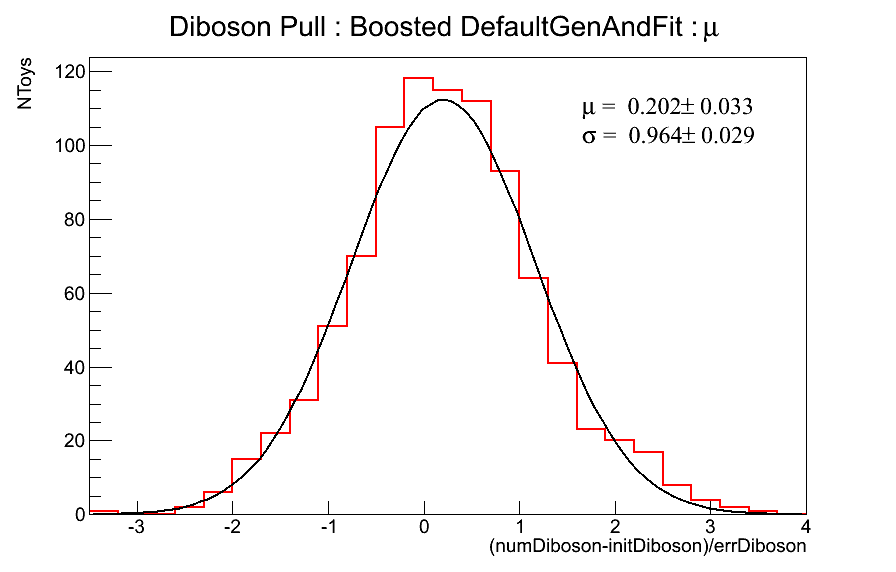
\includegraphics[width=0.48\textwidth]{figs/validation/Validation_DibosonPull_Boosted_mu.png}
\put(-0.80,0.0){(b)} \\ 
\unitlength=0.33\linewidth
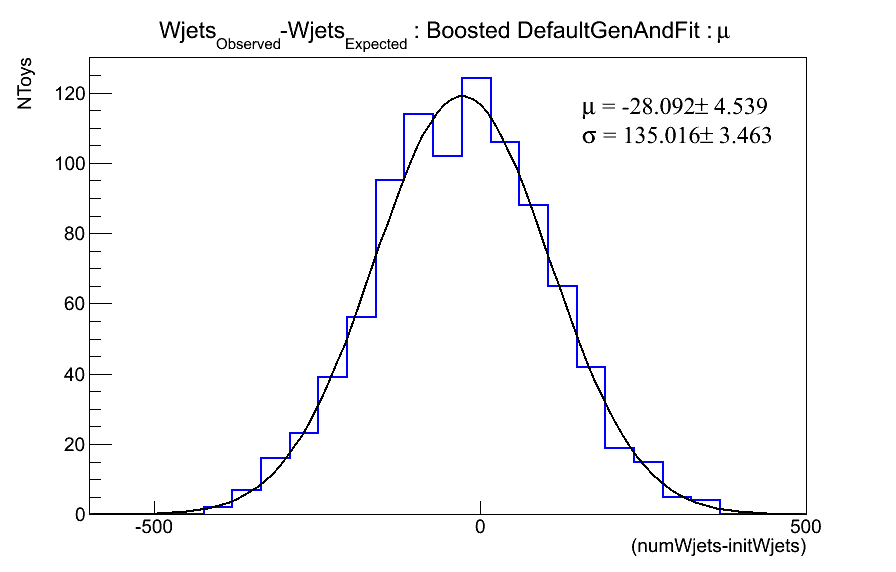
\includegraphics[width=0.48\textwidth]{figs/validation/Validation_WJetsYield_Boosted_mu.png}
\put(-0.80,0.0){(c)}
\unitlength=0.33\linewidth
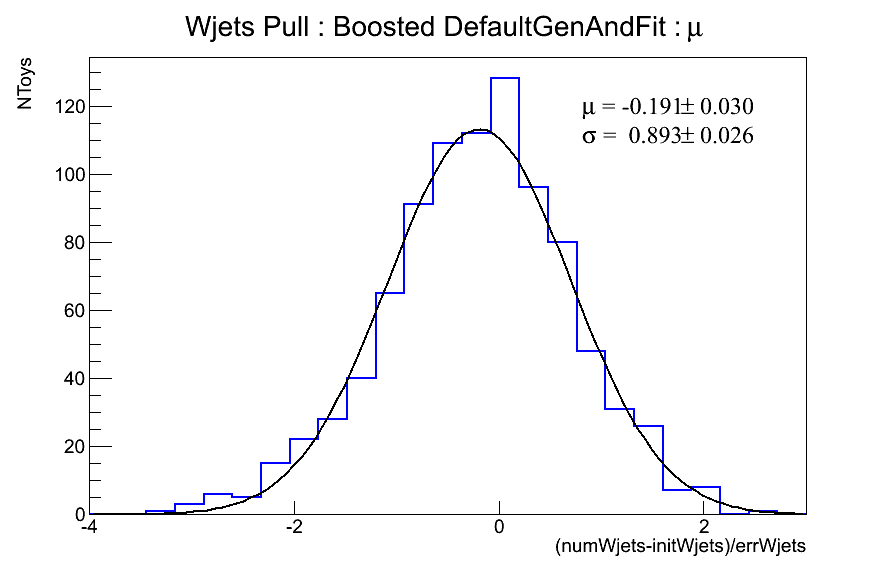
\includegraphics[width=0.48\textwidth]{figs/validation/Validation_WJetsPull_Boosted_mu.png}
\put(-0.80,0.0){(d)} \\ 
\unitlength=0.33\linewidth
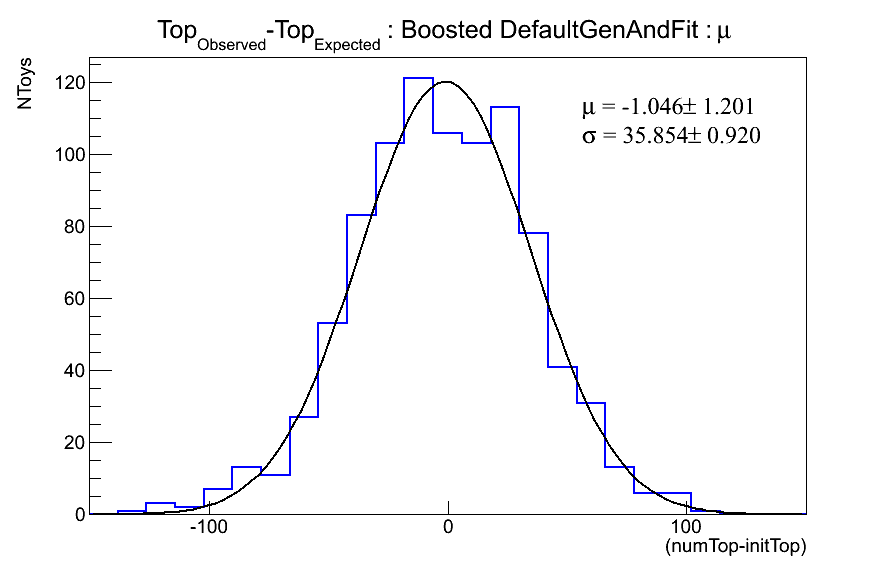
\includegraphics[width=0.48\textwidth]{figs/validation/Validation_topYield_Boosted_mu.png}
\put(-0.80,0.0){(e)}
\unitlength=0.33\linewidth
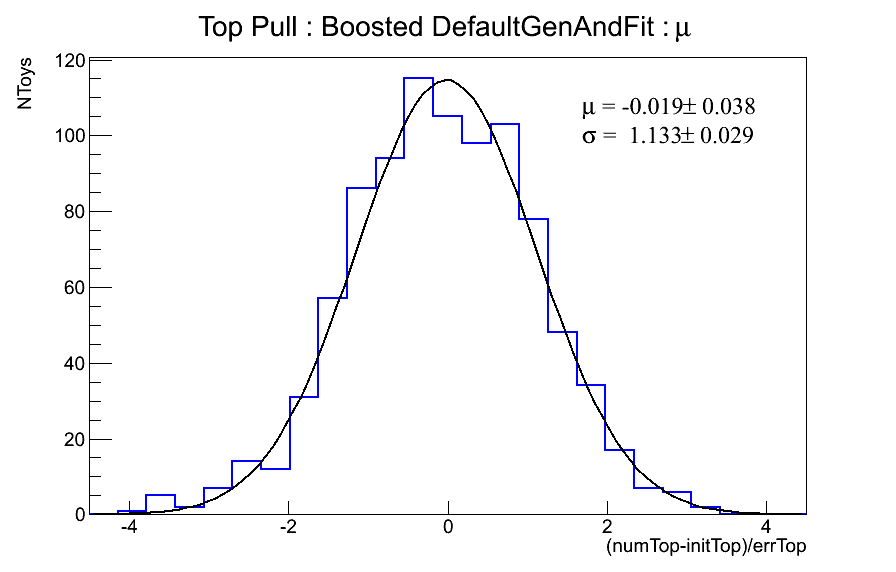
\includegraphics[width=0.48\textwidth]{figs/validation/Validation_topPull_Boosted_mu.png}
\put(-0.80,0.0){(f)}
\caption{Fit validation in the boosted muon channel, using 1000 Toy MC datasets. Fitted-Given yields for: (a) Diboson, (c) V+Jets, (e) top  and Pull=(Fitted-Given)/Error for: (b) Diboson, (d) V+Jets, (f) top.} 
\label{fig:Validation_mu_Boosted}}
\end{figure}
%%%%%%%
%%%%%%%
\begin{figure}[h!] {\centering
\unitlength=0.33\linewidth
\includegraphics[width=0.48\textwidth]{figs/validation/Validation_DibosonYield_Boosted_el.png}
\put(-0.80,0.0){(a)}
\unitlength=0.33\linewidth
\includegraphics[width=0.48\textwidth]{figs/validation/Validation_DibosonPull_Boosted_el.png}
\put(-0.80,0.0){(b)} \\ 
\unitlength=0.33\linewidth
\includegraphics[width=0.48\textwidth]{figs/validation/Validation_WJetsYield_Boosted_el.png}
\put(-0.80,0.0){(c)}
\unitlength=0.33\linewidth
\includegraphics[width=0.48\textwidth]{figs/validation/Validation_WJetsPull_Boosted_el.png}
\put(-0.80,0.0){(d)} \\ 
\unitlength=0.33\linewidth
\includegraphics[width=0.48\textwidth]{figs/validation/Validation_topYield_Boosted_el.png}
\put(-0.80,0.0){(e)}
\unitlength=0.33\linewidth
\includegraphics[width=0.48\textwidth]{figs/validation/Validation_topPull_Boosted_el.png}
\put(-0.80,0.0){(f)}
\caption{Fit validation in the boosted electron channel, using 1000 Toy MC datasets. Fitted-Given yields for: (a) Diboson, (c), (e) top V+Jets and Pull=(Fitted-Given)/Error for: (b) Diboson, (d) V+Jets, (f) top.} 
\label{fig:Validation_el_Boosted}}
\end{figure}
%%%%%%%
%%%%%%%%%%%%%%%%%%%%%%%%%

The fit biases for each channel are listed in Table~\ref{tab:SystematicCorrections}. On balance the fit configurations have a minor bias in the yield and overestimate the error by ~10-20\%. This is not unexpected since we do not know the precise parameterization for our background and compensate by using functions which (potentially) have more parameters than, what the 'true' form would contain. Furthermore, the high degree of correlation between the backgrounds (most notably V+Jets) and the diboson impacts its uncertainty. We use the above Yield and Pull distributions to correct for these effects.


\subsubsection{Fit Shape Validation}
Since we are relying on parametric shapes to model the data we need to ensure that the functional form used is sufficiently general and evaluate the corresponding error. First, we use alternate, more general, functional forms to fit the data. Then we generate toy datasets using the alternate form, but with the shape parameters obtained in the fits to the MC (rather than the data) and refit each dataset using the default configuration. {\it I.e.} we ensure that the alternate parametrization produces a good fit to the data, but compare one MC fit result to the other, since the objective is to ascertain the bias strictly due to the shape parameterization (the generated yield values are determined based on the default fit to the data by following the procedure described above). The results are shown in Figs.~\ref{fig:ShapeBias_mu_Standard},~\ref{fig:ShapeBias_el_Standard} for the anti-btagged dijet configuration, Figs.~\ref{fig:ShapeBias_mu_Btag},~\ref{fig:ShapeBias_el_Btag} for the btagged dijet configuration and in Figs.~\ref{fig:ShapeBias_mu_Boosted},~\ref{fig:ShapeBias_el_Boosted} for the boosted case.

%%%%%%%%%%%%%%%%%%%%%%%%%
%%%%%%%
\begin{figure}[h!] {\centering
\unitlength=0.33\linewidth
\includegraphics[width=0.48\textwidth]{figs/validation/ShapeBias_DibosonYield_Standard_mu.png}
\put(-0.80,0.0){(a)}
\unitlength=0.33\linewidth
\includegraphics[width=0.48\textwidth]{figs/validation/ShapeBias_DibosonPull_Standard_mu.png}
\put(-0.80,0.0){(b)} \\ 
\unitlength=0.33\linewidth
\includegraphics[width=0.48\textwidth]{figs/validation/ShapeBias_WJetsYield_Standard_mu.png}
\put(-0.80,0.0){(c)}
\unitlength=0.33\linewidth
\includegraphics[width=0.48\textwidth]{figs/validation/ShapeBias_WJetsPull_Standard_mu.png}
\put(-0.80,0.0){(d)} 
\caption{Shape validation in the (anti-btagged) dijet the muon channel, using 1000 Toy MC datasets. Fitted-Given yields for: (a) Diboson, (c) V+Jets and Pull=(Fitted-Given)/Error for: (b) Diboson, (d) V+Jets.} 
\label{fig:ShapeBias_mu_Standard}}
\end{figure}
%%%%%%%
%%%%%%%
\begin{figure}[h!] {\centering
\unitlength=0.33\linewidth
\includegraphics[width=0.48\textwidth]{figs/validation/ShapeBias_DibosonYield_Standard_el.png}
\put(-0.80,0.0){(a)}
\unitlength=0.33\linewidth
\includegraphics[width=0.48\textwidth]{figs/validation/ShapeBias_DibosonPull_Standard_el.png}
\put(-0.80,0.0){(b)} \\ 
\unitlength=0.33\linewidth
\includegraphics[width=0.48\textwidth]{figs/validation/ShapeBias_WJetsYield_Standard_el.png}
\put(-0.80,0.0){(c)}
\unitlength=0.33\linewidth
\includegraphics[width=0.48\textwidth]{figs/validation/ShapeBias_WJetsPull_Standard_el.png}
\put(-0.80,0.0){(d)} 
\caption{Shape validation in the (anti-btagged) dijet the electron channel, using 1000 Toy MC datasets. Fitted-Given yields for: (a) Diboson, (c) V+Jets and Pull=(Fitted-Given)/Error for: (b) Diboson, (d) V+Jets.} 
\label{fig:ShapeBias_el_Standard}}
\end{figure}
%%%%%%%
\begin{figure}[h!] {\centering
\unitlength=0.33\linewidth
\includegraphics[width=0.48\textwidth]{figs/validation/ShapeBias_DibosonYield_Btag_mu.png}
\put(-0.80,0.0){(a)}
\unitlength=0.33\linewidth
\includegraphics[width=0.48\textwidth]{figs/validation/ShapeBias_DibosonPull_Btag_mu.png}
\put(-0.80,0.0){(b)} \\ 
\unitlength=0.33\linewidth
\includegraphics[width=0.48\textwidth]{figs/validation/ShapeBias_WJetsYield_Btag_mu.png}
\put(-0.80,0.0){(c)}
\unitlength=0.33\linewidth
\includegraphics[width=0.48\textwidth]{figs/validation/ShapeBias_WJetsPull_Btag_mu.png}
\put(-0.80,0.0){(d)} \\
\unitlength=0.33\linewidth
\includegraphics[width=0.48\textwidth]{figs/validation/ShapeBias_topYield_Btag_mu.png}
\put(-0.80,0.0){(e)}
\unitlength=0.33\linewidth
\includegraphics[width=0.48\textwidth]{figs/validation/ShapeBias_topPull_Btag_mu.png}
\put(-0.80,0.0){(f)} 
\caption{Shape validation in the (anti-btagged) dijet the muon channel, using 1000 Toy MC datasets. Fitted-Given yields for: (a) Diboson, (c) V+Jets, (e) top and Pull=(Fitted-Given)/Error for: (b) Diboson, (d) V+Jets, (f) top.} 
\label{fig:ShapeBias_mu_Btag}}
\end{figure}
%%%%%%%
%%%%%%%
\begin{figure}[h!] {\centering
\unitlength=0.33\linewidth
\includegraphics[width=0.48\textwidth]{figs/validation/ShapeBias_DibosonYield_Btag_el.png}
\put(-0.80,0.0){(a)}
\unitlength=0.33\linewidth
\includegraphics[width=0.48\textwidth]{figs/validation/ShapeBias_DibosonPull_Btag_el.png}
\put(-0.80,0.0){(b)} \\ 
\unitlength=0.33\linewidth
\includegraphics[width=0.48\textwidth]{figs/validation/ShapeBias_WJetsYield_Btag_el.png}
\put(-0.80,0.0){(c)}
\unitlength=0.33\linewidth
\includegraphics[width=0.48\textwidth]{figs/validation/ShapeBias_WJetsPull_Btag_el.png}
\put(-0.80,0.0){(d)} \\
\unitlength=0.33\linewidth
\includegraphics[width=0.48\textwidth]{figs/validation/ShapeBias_topYield_Btag_el.png}
\put(-0.80,0.0){(e)}
\unitlength=0.33\linewidth
\includegraphics[width=0.48\textwidth]{figs/validation/ShapeBias_topPull_Btag_el.png}
\put(-0.80,0.0){(f)} 
\caption{Shape validation in the (anti-btagged) dijet the electron channel, using 1000 Toy MC datasets. Fitted-Given yields for: (a) Diboson, (c) V+Jets, (e) top and Pull=(Fitted-Given)/Error for: (b) Diboson, (d) V+Jets, (f) top.} 
\label{fig:ShapeBias_el_Btag}}
\end{figure}
%%%%%%%
%%%%%%%
\begin{figure}[h!] {\centering
\unitlength=0.33\linewidth
\includegraphics[width=0.48\textwidth]{figs/validation/ShapeBias_DibosonYield_Boosted_mu.png}
\put(-0.80,0.0){(a)}
\unitlength=0.33\linewidth
\includegraphics[width=0.48\textwidth]{figs/validation/ShapeBias_DibosonPull_Boosted_mu.png}
\put(-0.80,0.0){(b)} \\ 
\unitlength=0.33\linewidth
\includegraphics[width=0.48\textwidth]{figs/validation/ShapeBias_WJetsYield_Boosted_mu.png}
\put(-0.80,0.0){(c)}
\unitlength=0.33\linewidth
\includegraphics[width=0.48\textwidth]{figs/validation/ShapeBias_WJetsPull_Boosted_mu.png}
\put(-0.80,0.0){(d)} \\ 
\unitlength=0.33\linewidth
\includegraphics[width=0.48\textwidth]{figs/validation/ShapeBias_topYield_Boosted_mu.png}
\put(-0.80,0.0){(e)}
\unitlength=0.33\linewidth
\includegraphics[width=0.48\textwidth]{figs/validation/ShapeBias_topPull_Boosted_mu.png}
\put(-0.80,0.0){(f)} 
\caption{Shape validation in the boosted muon channel, using 1000 Toy MC datasets. Fitted-Given yields for: (a) Diboson, (c) V+Jets, (e) top and Pull=(Fitted-Given)/Error for: (b) Diboson, (d) V+Jets, (f) top.} 
\label{fig:ShapeBias_mu_Boosted}}
\end{figure}
%%%%%%%
%%%%%%%
\begin{figure}[h!] {\centering
\unitlength=0.33\linewidth
\includegraphics[width=0.48\textwidth]{figs/validation/ShapeBias_DibosonYield_Boosted_el.png}
\put(-0.80,0.0){(a)}
\unitlength=0.33\linewidth
\includegraphics[width=0.48\textwidth]{figs/validation/ShapeBias_DibosonPull_Boosted_el.png}
\put(-0.80,0.0){(b)} \\ 
\unitlength=0.33\linewidth
\includegraphics[width=0.48\textwidth]{figs/validation/ShapeBias_WJetsYield_Boosted_el.png}
\put(-0.80,0.0){(c)}
\unitlength=0.33\linewidth
\includegraphics[width=0.48\textwidth]{figs/validation/ShapeBias_WJetsPull_Boosted_el.png}
\put(-0.80,0.0){(d)} \\ 
\unitlength=0.33\linewidth
\includegraphics[width=0.48\textwidth]{figs/validation/ShapeBias_topYield_Boosted_el.png}
\put(-0.80,0.0){(e)}
\unitlength=0.33\linewidth
\includegraphics[width=0.48\textwidth]{figs/validation/ShapeBias_topPull_Boosted_el.png}
\put(-0.80,0.0){(f)} 
\caption{Shape validation in the boosted electron channel, using 1000 Toy MC datasets. Fitted-Given yields for: (a) Diboson, (c) V+Jets, (e) top and Pull=(Fitted-Given)/Error for: (b) Diboson, (d) V+Jets, (f) top.} 
\label{fig:ShapeBias_el_Boosted}}
\end{figure}
%%%%%%%
%%%%%%%%%%%%%%%%%%%%%%%%%

As can be seen there is an (up to ~20\%) bias between the given and fitted yields. We account for it by adding the offset in the number of events (in quadrature) to the total error. The diboson yields after correcting for (all of) the corresponding biases are listed in Table~\ref{table:FitTotalsAndComparisons}.

%%%%%%%%%%%%%%%%%%%%%%%%%%%%%%%%%%%%%%%%%%%%%%%%%%%%%%%%%%%%
\subsection{Total Cross Section}
    Combining the six channels (in Table~\ref{tab:SystematicCorrections}) gives a total of $9330.5\pm 1102.4$ diboson events. %with a $7.3\sigma$ significance. 
Upon correcting for biases in the extracted yield and corresponding error as well as shape systematics, we extract $9233.8\pm 1059.7$ WW+WZ events. The diboson cross section is computed for each of the six channels as $\sigma = N_{\text{Sig}}/ (\mathcal{A} \, \varepsilon \, {\mathcal{L}})$, where $N_{\text{Sig}}$ is the number of extracted signal events, $\mathcal{A}$ is the signal acceptance corrected for the branching fractions, $\varepsilon$ is the overall efficiency for event selection (listed for each channel in Table~\ref{tab:signals}), ${\mathcal{L}}$ is the integrated luminosity. The results are listed in Table~\ref{tab:dibosonYield}. We combine the individual cross-sections by assining each a weight proportional to the inverse of the uncertainty squared, effectively minimizing the $\chi^2$ of the fit (to the cross-section values with a constant). An additional systematic uncertainty (total, without luminosity in Table~\ref{tab:signalSyst}) is added in quadrature to the systematic error. The Luminosity uncertainty (Section~\ref{sec:LumiUncertainty}) is included separately. The total cross section is $126.2 \pm 7.8\text{(stat)} \pm 13.9\text{(syst)} \pm 3.3\text{(lumi)}$~pb, statistically consitent with the individual channel results as well as the Standard Model expectation of $80.1^{+2.51}_{-1.74}\unit{pb}$~\cite{Campbell:2011bn} (with a summary of the measurements shown in Fig.~\ref{fig:CrossSectionSummary}).


%%%%%%%%%%%%%%%%%%%%%%%%%%%%
%%%%%%%
\begin{figure}[h!] {\centering
\unitlength=0.33\linewidth
\includegraphics[width=0.90\textwidth]{figs/WW_WZ_crossX_6chan_8TeV.png}
\caption{Measured cross sections for each of the six channels, combined total and the theory prediction.}
\label{fig:CrossSectionSummary}}
\end{figure}
%%%%%%%
%%%%%%%%%%%%%%%%%%%%%%%%%%%%